\documentclass[a4paper,12pt]{article}
\usepackage{color}
\usepackage{graphicx}
\usepackage{listings}

\usepackage{hyperref}

\usepackage{float}

\begin{document}

\title{Bhargava Design Handbook}
\author{Aman Bhargava}
\date{\today}
\maketitle

\tableofcontents

\section{Identity}
\subsection{A Brief Biography}
My name is Aman Bhargava, and I am currently an Engineering Science student at the University of Toronto. I was born and raised in the state of Maine in the United States, and I moved to Cobourg, Ontario when I was 12.

\subsection{My Values}
I value altruism, creativity/open-mindedness, efficiency, and practicality. Figure 1 represents the flowchart of goodness I see these forming.

\begin{figure}[H]
\centering
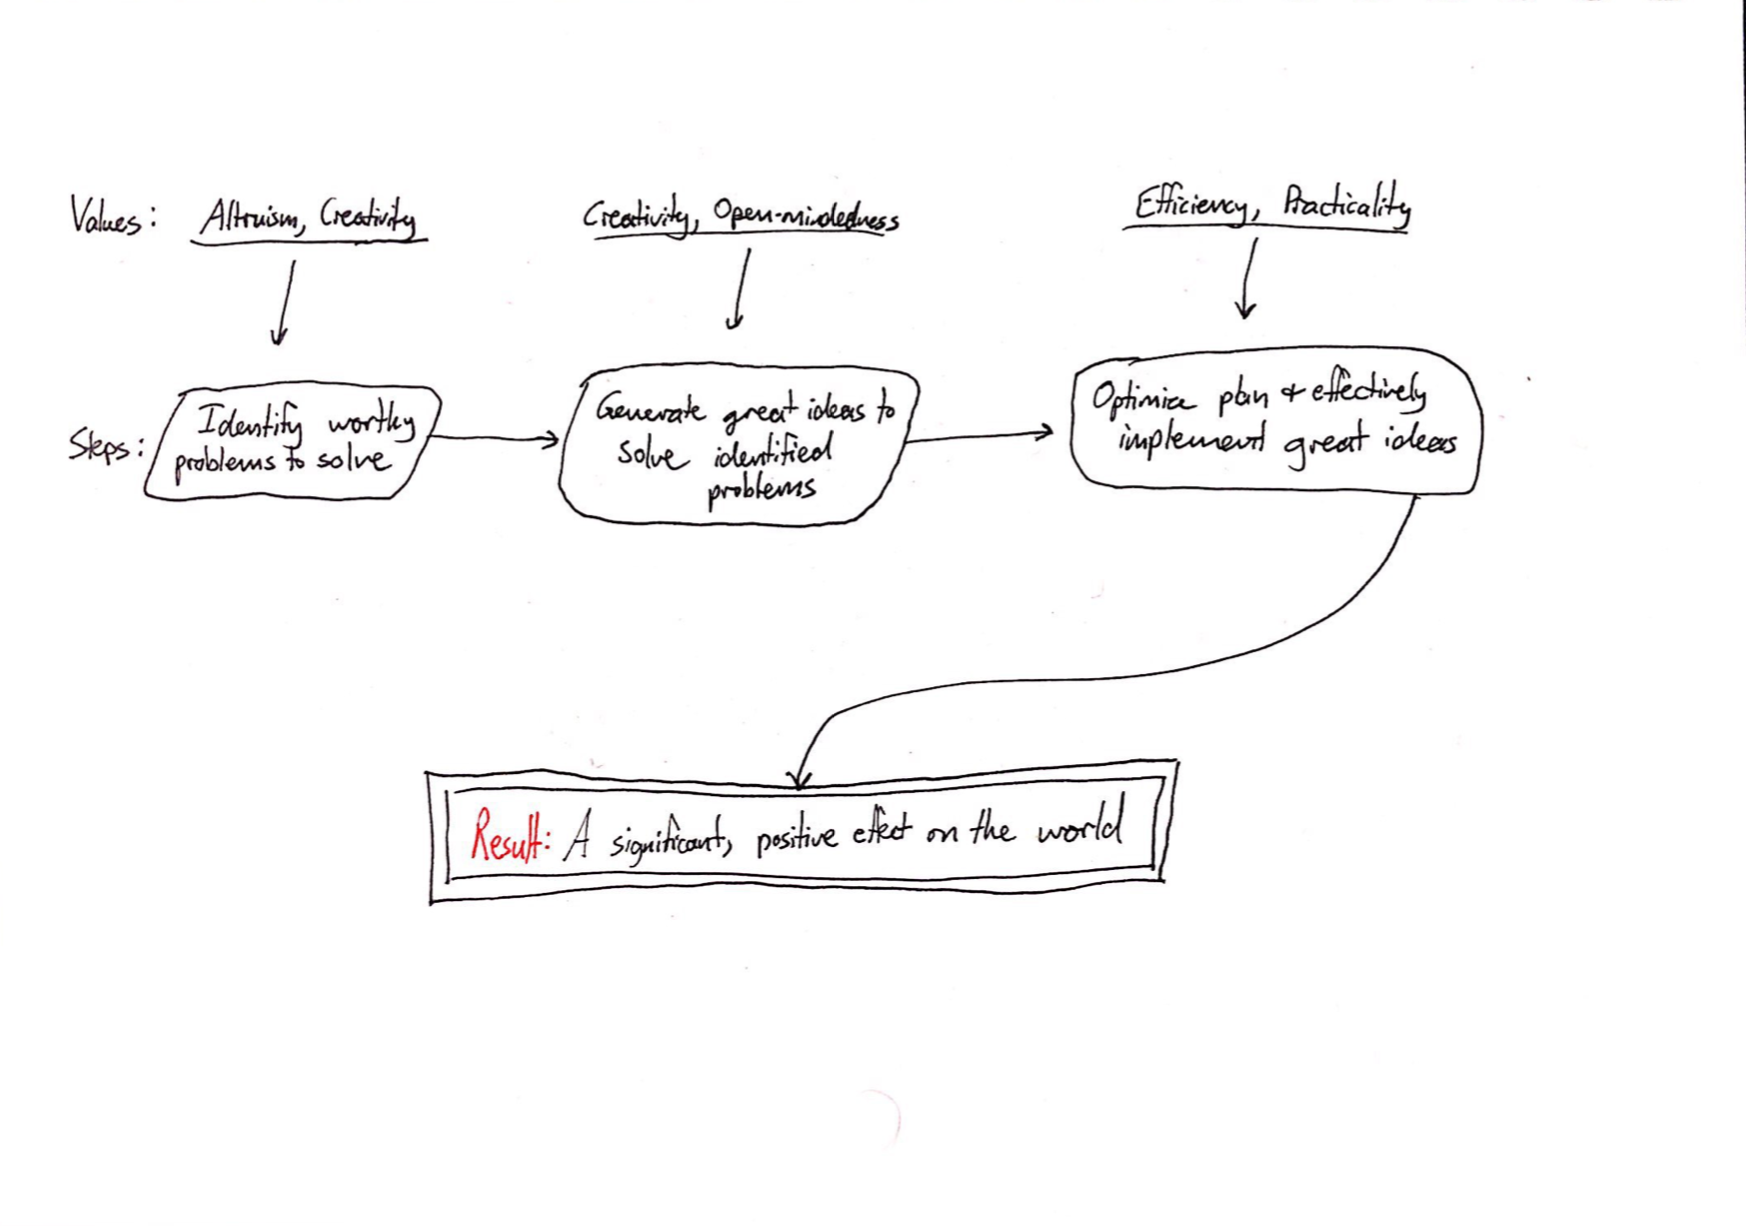
\includegraphics[width=0.9\textwidth]{img/image001.png}
\caption{How my values integrate with the steps to my goal of significantly and positively changing the world.}
\label{}
\end{figure}

I believe that this general cycle has the power to have a significant and positive effect on the world, which is one of my most deeply-held ambitions in life.

\subsection{Skills}
\begin{enumerate}
\item Team organization and leadership: Through my experience in leading group projects in school, university, hackathons and more, I have learned how to run an effective, goal-driven team.
\item Programming: I have confidence in my ability to implement ideas into software, at least in such a way that can communicate a basic idea.
\item Data Analysis: I am competent with data visualization, basic statistics, supervised machine learning, and basic clustering.
\item Fabrication: I am competent with basic fabrication tools, namely those found in the Light Fabrication Facility (3D-printing, laser cutting, foam core, basic carpentry, arduino/raspberry pi programming)
\item Argumentation: As a former provincial debater, I believe in my ability to effectively use argumentation to get closer to the truth in the vast majority of issues that I am able to understand.
\item Research: I am able to effectively utilize engineering and scholarly libraries and databases to get the information that I need.
\item Self-learning: My ability to learn things as needed on my own has proven useful time and time again in all of my projects.
\end{enumerate}

\subsection{Biases}
Everything I have written so far in this introduction is a potential bias. Due to my experience in programming, I am likely overly willing to go down the technological route to solve problems without considering non-technological solutions. Because I pride myself in my ability to teach myself, I am less likely than would be optimal to ask for help or consider the possibility of a project being out of my abilities.

Beyond the biases I have implicitly defined in this introduction, I think that my personality makes me overly willing to go outside the box for projects. Because I value creativity so highly, I find it boring to go by the book and am susceptible to the temptation of going outside the box even when it might not be favourable for the design objective.

More generally, I am biased by what I think is “boring” and “interesting”. Even when I try not to, one of the first things I think of when I consider a design alternative or process idea is how “cool” it seems. Even if an alternative will meet the needs of our requirements model/our stakeholders’ needs, I will be turned off of it if it doesn’t meet my subjective, unconscious criteria for what is “interesting”.

Finally, I have been in private schools for my entire life. Simultaneously, I have frequently visited my parent’s home country of India, where I have been exposed (for several weeks at a time) to extreme poverty. I have most of my time around two ends of the socio-economic spectrum, and I am almost certainly biased by that extremism, though I find it difficult to predict exactly how.

\subsection{Metadiscourse on Handbook Design}
I will go on to discuss my projects, including the process followed and holistic review for each, followed by a description and justification of my personal design process, and finally a full overview of all the tools, models, and frameworks mentioned and briefly discussed in the projects section.

My handbook is organized this way because my projects are a core part of my identity and therefore ought to be introduced first to better understand my use of tools and the derivation of my personal design process. I choose to be detailed about my projects because, in my experience in writing guides for my future self, I require many mental hooks to draw upon in order to recall concepts, ideas, and skills optimally.

This organization also mirrors my value system organization. I introduce my projects (i.e. ‘identifying worthy problems to solve’), then my personal design process (i.e. a tool to ‘generate creative, good solutions to these problems’), and finally close with detailed description of each engineering design tool (i.e. methods to ‘optimize my plan and effectively implement the great ideas’).

I chose not to group my Tools into categories such as FDCR because I invented many of them and many are from outside of Praxis lectures, so they don’t fit directly into easily describable categories. As well, when I am looking through in the future, being forced to look through all my favourite tools will help me to potentially creatively alter a tool that wouldn’t initially fit the use case, but could both my project via its effectiveness and actualize my values of creativity and open mindedness.

My invented tools are valid because I have evidence in the form of my experience that they work for me. Since this handbook is meant for my future design work, I am a key stakeholder and that it plenty of reason to be valid. On top of this, I incorporate further research to justify why many of my invented tools are valid.




\section{Projects}
\subsection{Importance of Projects}
I have always been a project-oriented person, and I love doing projects. Using projects as case studies has been extremely valuable for my success in later projects. The following is a brief summation of some of my projects from the past year, since the beginning of Praxis I. I will present them in chronological order, discussing the project goals, process, and a brief holistic review.

\subsection{Praxis I Design - Smart Hat}
For our Praxis I design project, Alice, Kelvin and I worked to improve the quality of sleep for Engsci’s in transit. We designed for effectiveness in terms of light and sound blockage, along with cost, comfort, durability, and aesthetics.

\subsubsection{Process}
We diverged a multitude of ideas using tools such as \textbf{extreme DfX} and then converged to a conceptual design via \textbf{system 1.5 analysis} and comparing our alternatives using high-level objectives via \textbf{logical argumentation and research}. We built a low-fidelity prototype using a Santa hat and a pair of cheap headphones to demonstrate our idea and to get a sense of the scale. Then, we used the \textbf{divide and conquer} design tool to divide our design exercise into many smaller design problems and did smaller rounds of framing, diverging, and converging for each detailed design decision. This enabled us to turn our conceptual design into a detailed, well-substantiated design.

\begin{figure}[H]
\centering
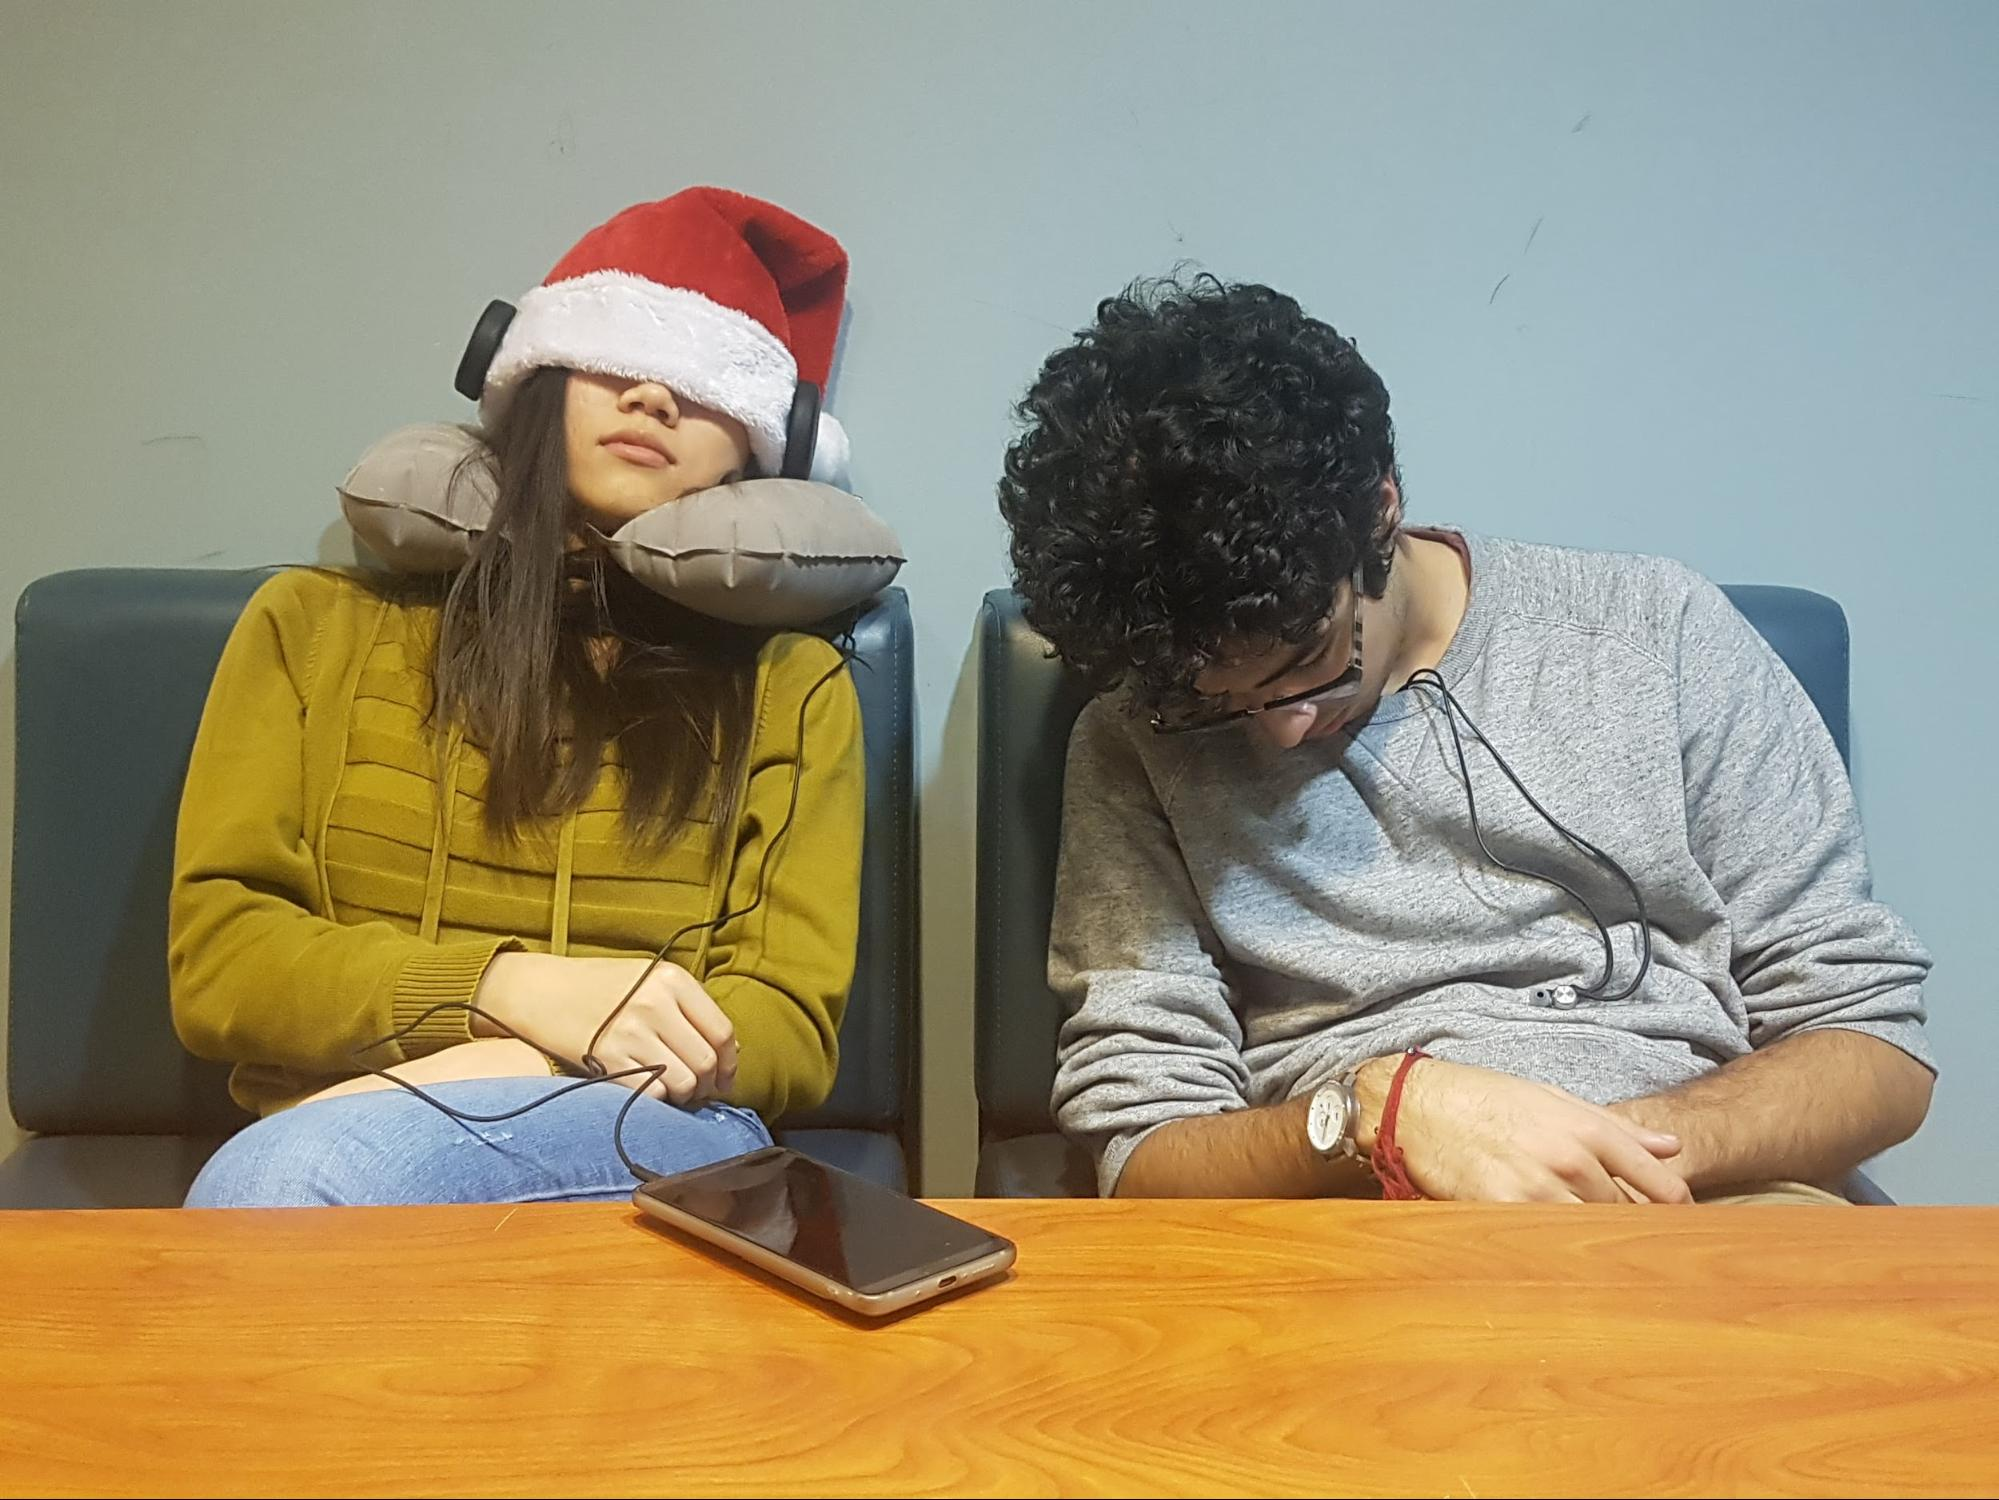
\includegraphics[width=1\textwidth]{img/image002.jpg}
\caption{Demonstrating beta prototype. Our final design retained the shape presented but used \textbf{divide and conoquer} to add rigour to the fine details.}
\label{}
\end{figure}

\begin{figure}[H]
\centering
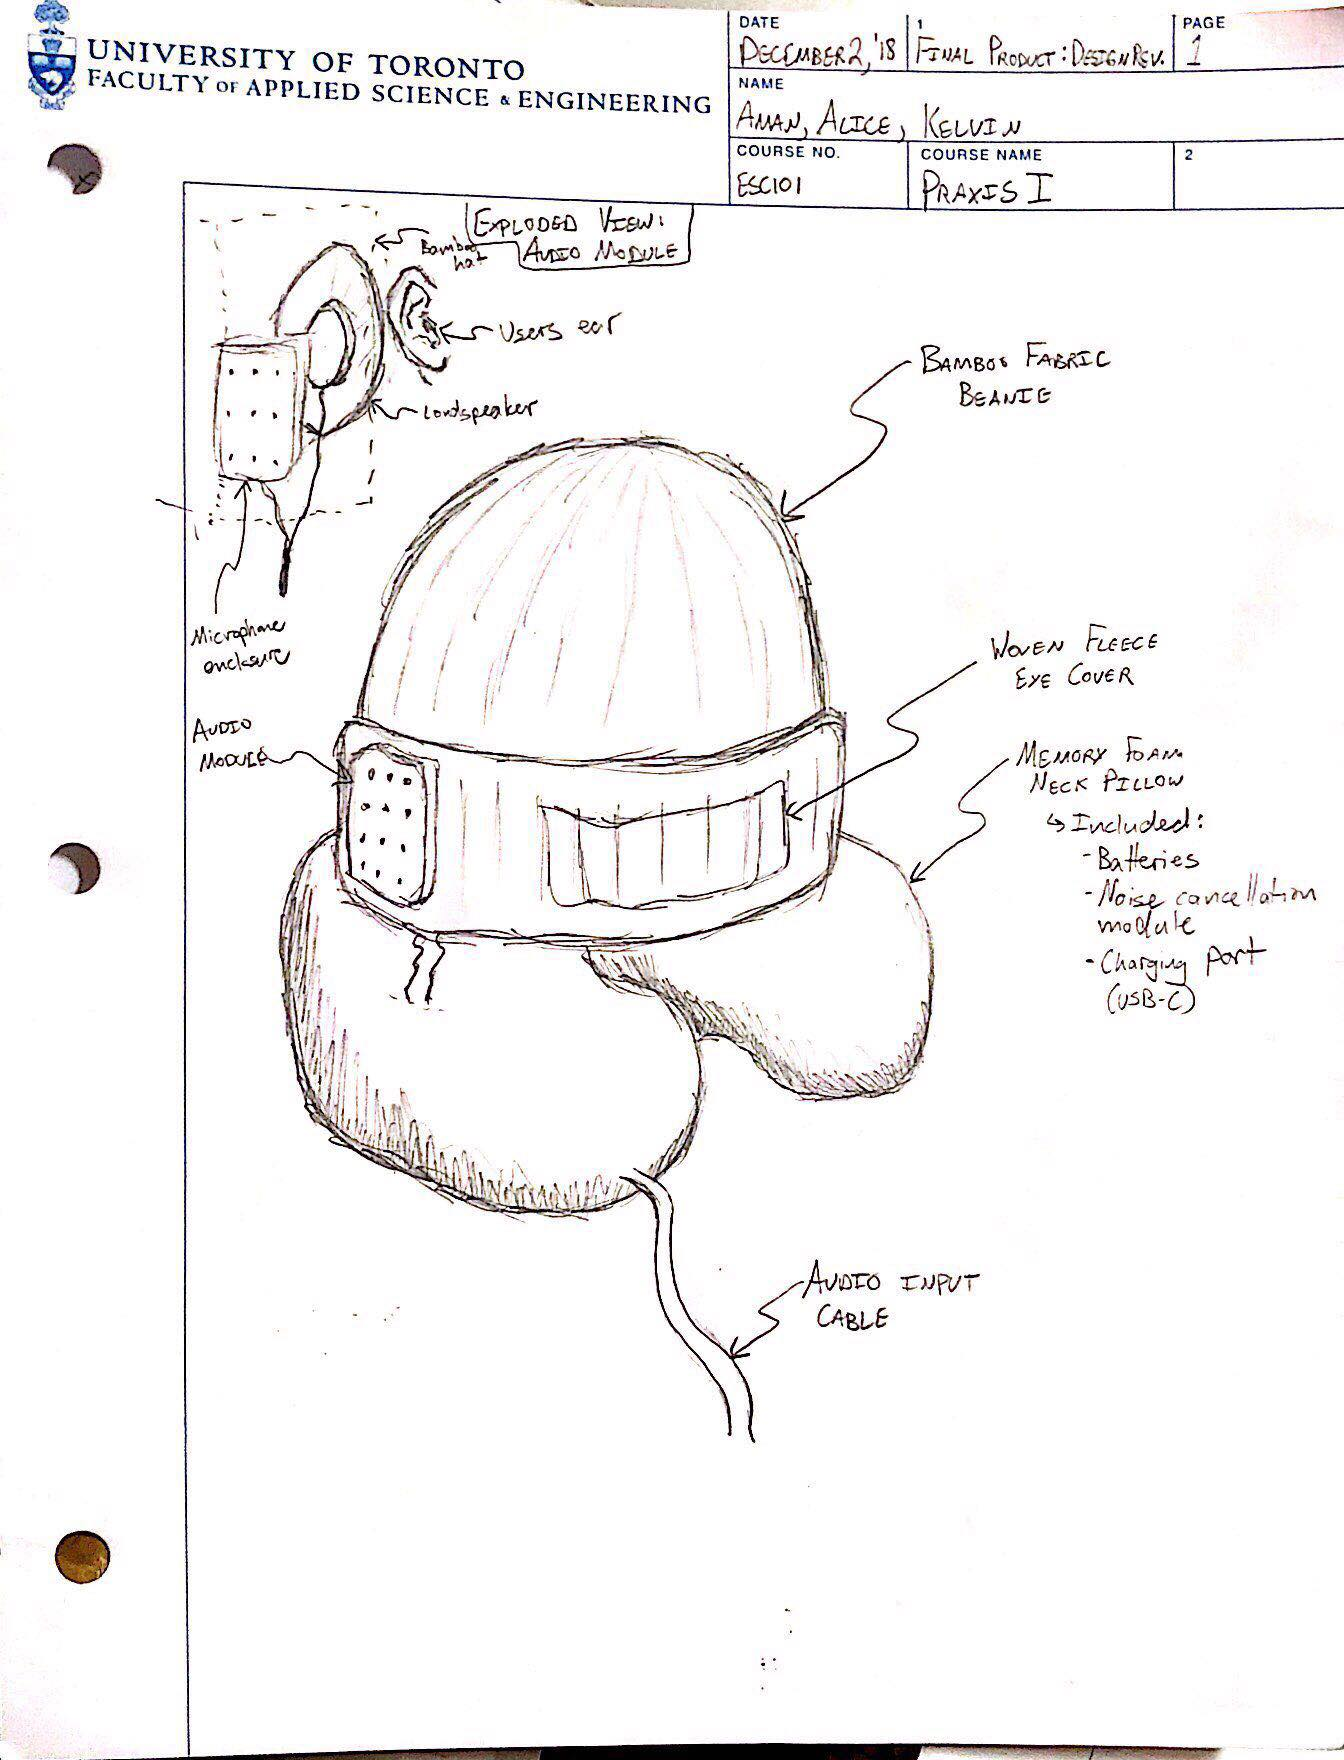
\includegraphics[width=1\textwidth]{img/image003.jpg}
\caption{Our final design, post divide and conquer. The design is far more specific and rigorous than the beta version, but is remains informed by the initial design.}
\label{}
\end{figure}

\subsubsection{Holistic Review}
Overall, I believe that we made a well-argued case for our design. We had comprehensive research and strong prototyping, but I believe that we were rather held back by our attachment to dogmatic design. We were concerned more about the quality of our grades rather than the quality of our designs. Because of this, we were overly attached to the design process discussed in class. We initially did not realize that we were allowed to break our design decision into multiple smaller design decisions. Because of this, we thought that we would need to go through a tremendous number of fully-fledged alternatives in order to arrive at a ‘well justified’ final design. It was only after I drafted this alternative journey 3 days before the due date that we were able to really move forward well.

The biggest lesson learned was that the design process is malleable. If one can come up with a good reason to change the design process to better fit the opportunity at hand, it is their duty as an engineer to at least argue for that change in the design process.

\begin{figure}[H]
\centering
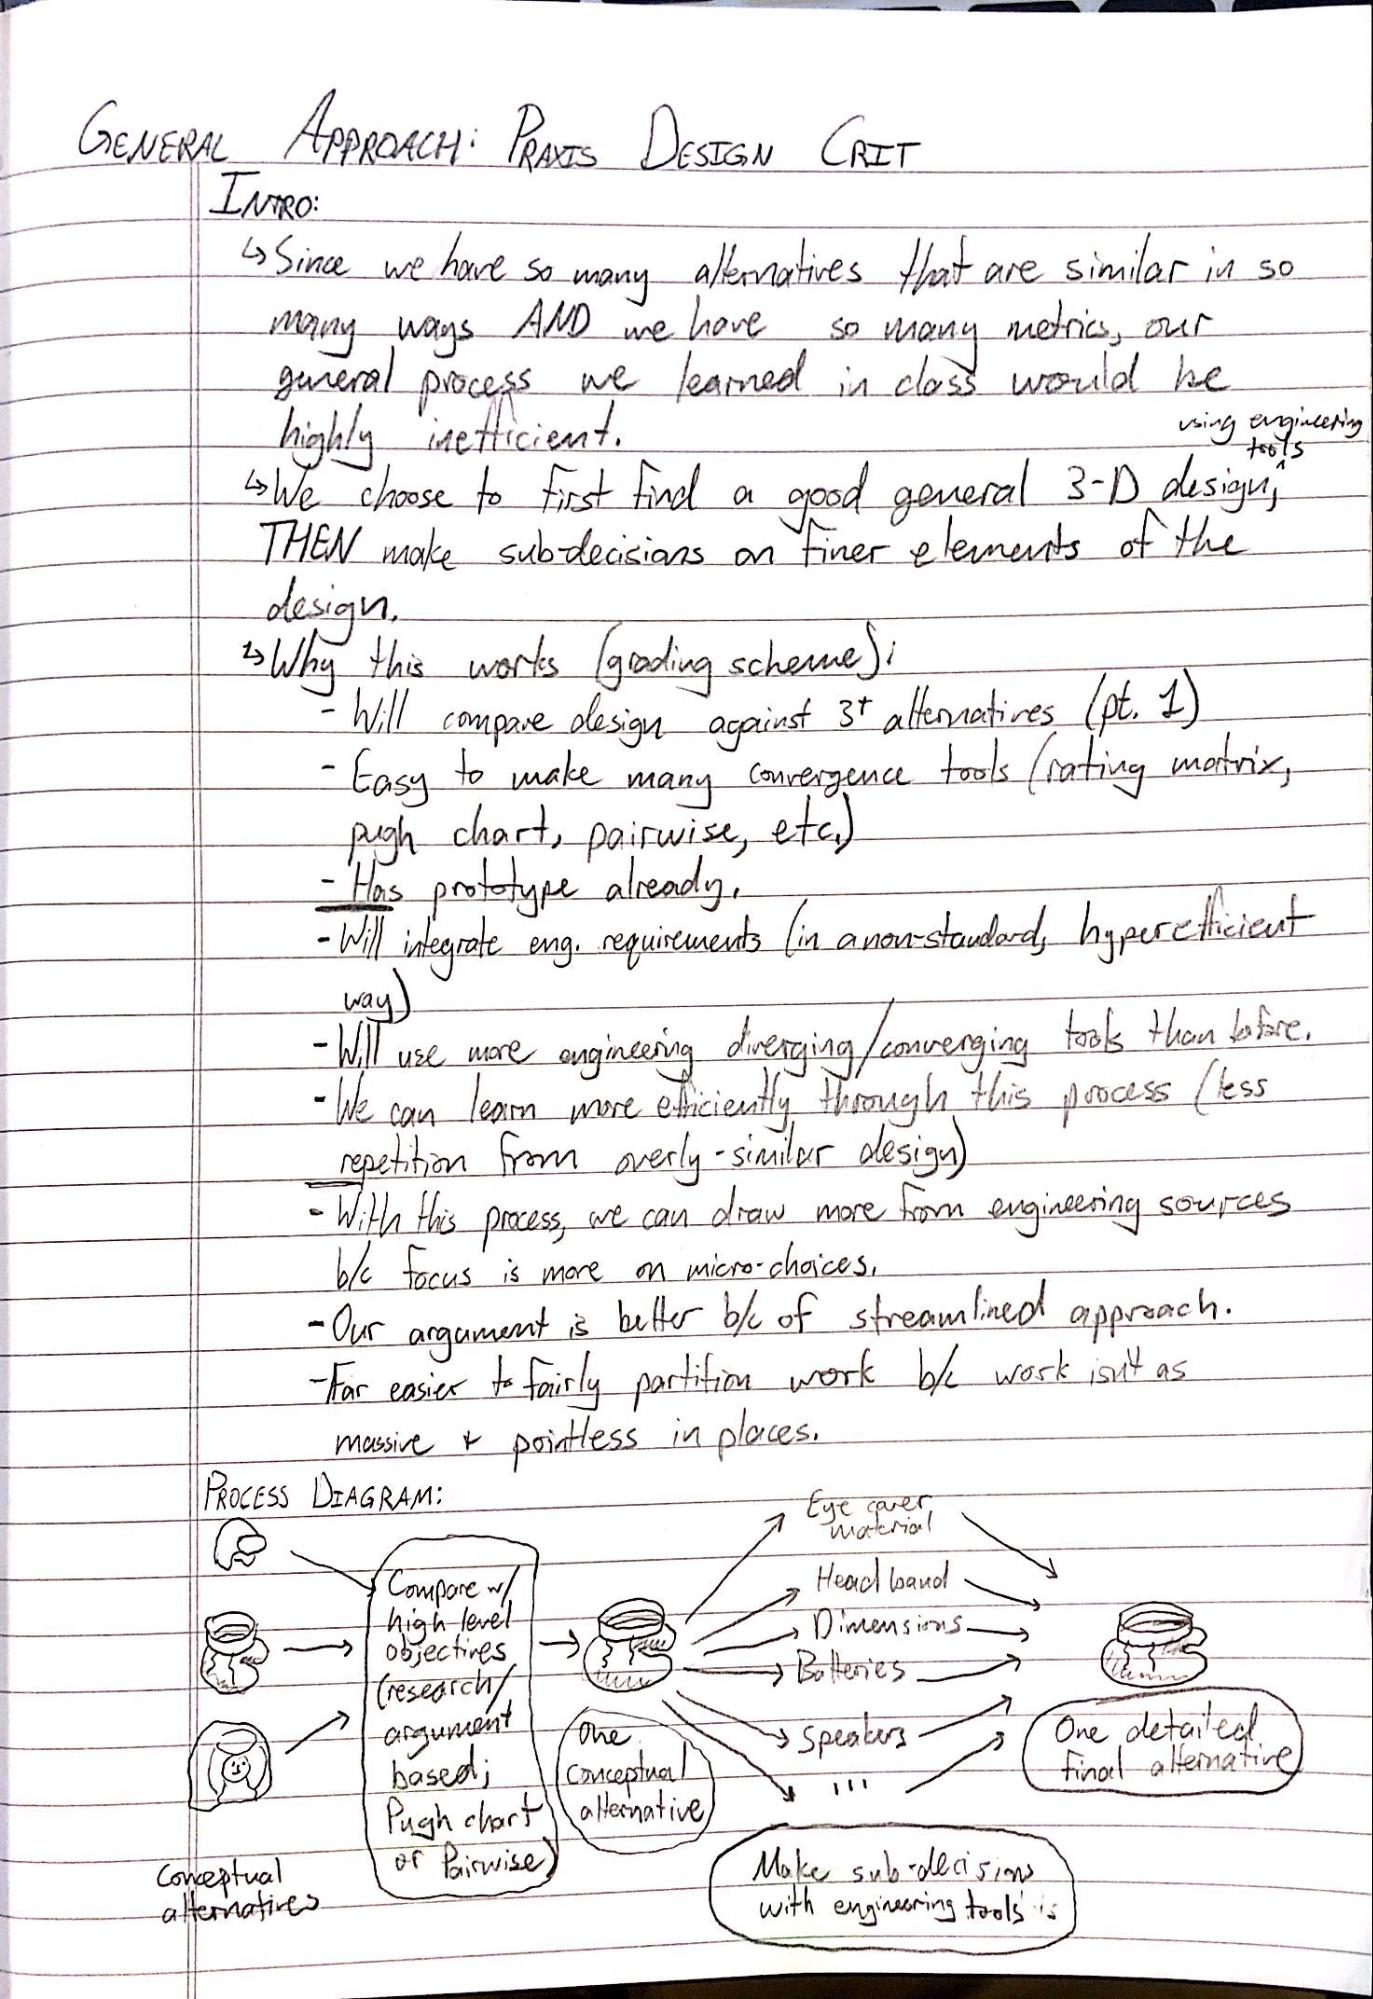
\includegraphics[width=1\textwidth]{img/image004.jpg}
\caption{My initial proposal for the group to use the 'divide and conquer' method to finalize our design. The experience of changing the design process influenced the rest of my projects and my personal design process profoundly.}
\label{}
\end{figure}


\subsection{CIV102 - Genetic Bridge Algorithm}
The CIV102 bridge project is a staple of Engsci, but my biggest takeaway from it was a ‘side project’ of sorts that stemmed from the main project. We were tasked with making a matboard bridge that could hold the maximum amount of weight under some specified loading conditions. In class, we learned the formulae that would give the amount of weight a bridge would hold before failing by some arbitrary failure mechanism.

\subsubsection{Process}

As soon as I saw this assignment, I saw how it could easily be made into an optimization problem; the project had clear objective functions (formulae for failure loading), constraints (amount of matboard) and structure (a bridge). After discussing with our team, we decided it would be in our best interest if I were to take the time to code our bridge measurement formulae and attempt to make an optimization algorithm to generate the parameters for our bridge design. We came to this decision via an \textbf{expected value calculation} - we looked at the potential benefit to our grade (25\% bonus for ‘creative solutions’) and my chances of success (estimated fairly high given my background in programming and genetic algorithms).

I chose a genetic algorithm because it mirrors the design process that Professor Collins teaches - it is literally a \textbf{rapid, (automated) iterative design process}. This worked fantastically well in creating extremely strong bridge designs (designs predicted to withstand more than 3 kilonewtons), and our group was still able to do well despite the fact we struggled with implementing the design due to the fact that we managed the risk well (performed \textbf{expected value calculations}).

\begin{figure}[H]
\centering
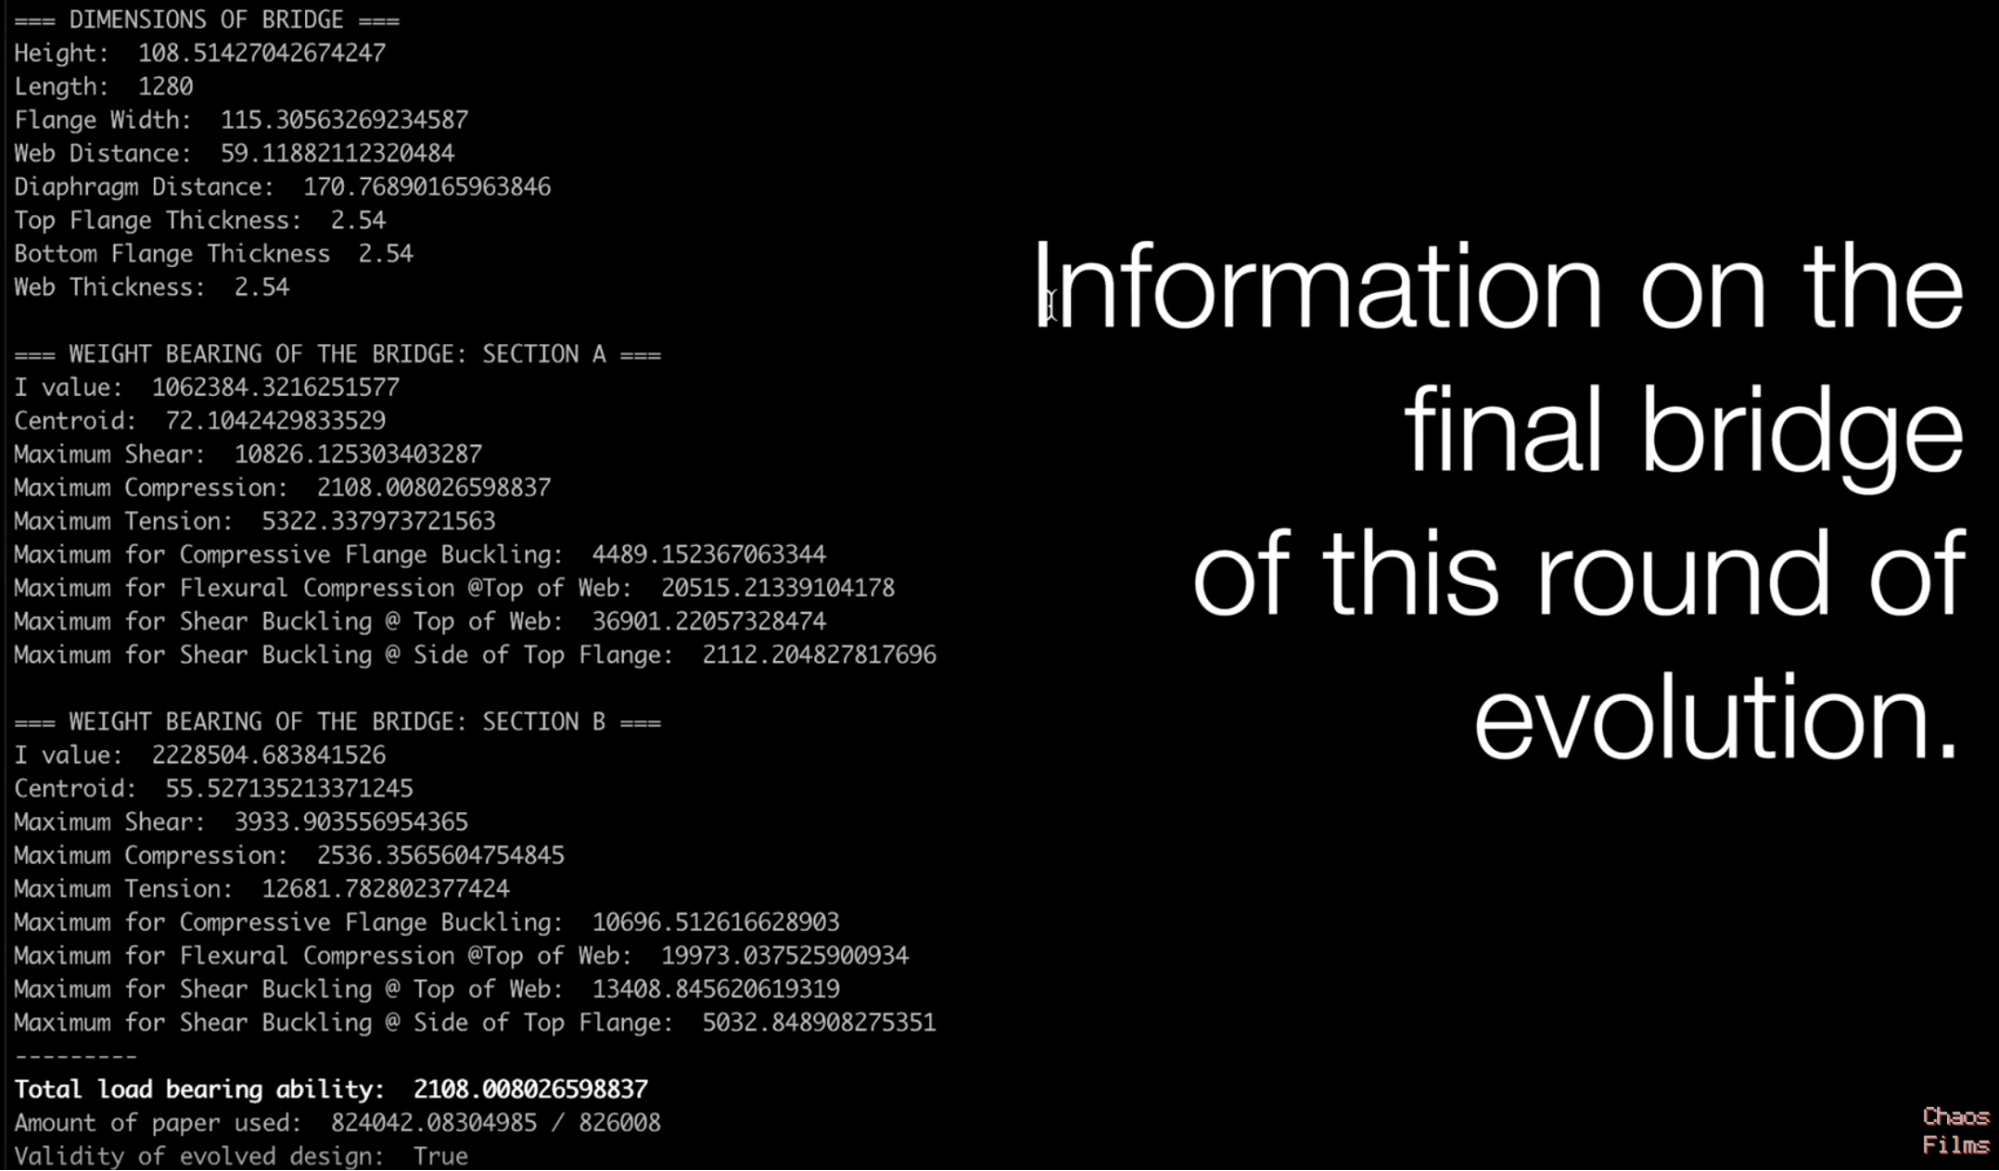
\includegraphics[width=0.7\textwidth]{img/image005.png}
\caption{The output of the evolution program. This improved our \textbf{expected value calculations} because we could test it against our paper calculations easily and trace bugs in the code back to their functions based on this output.}
\label{}
\end{figure}

\begin{figure}[H]
\centering
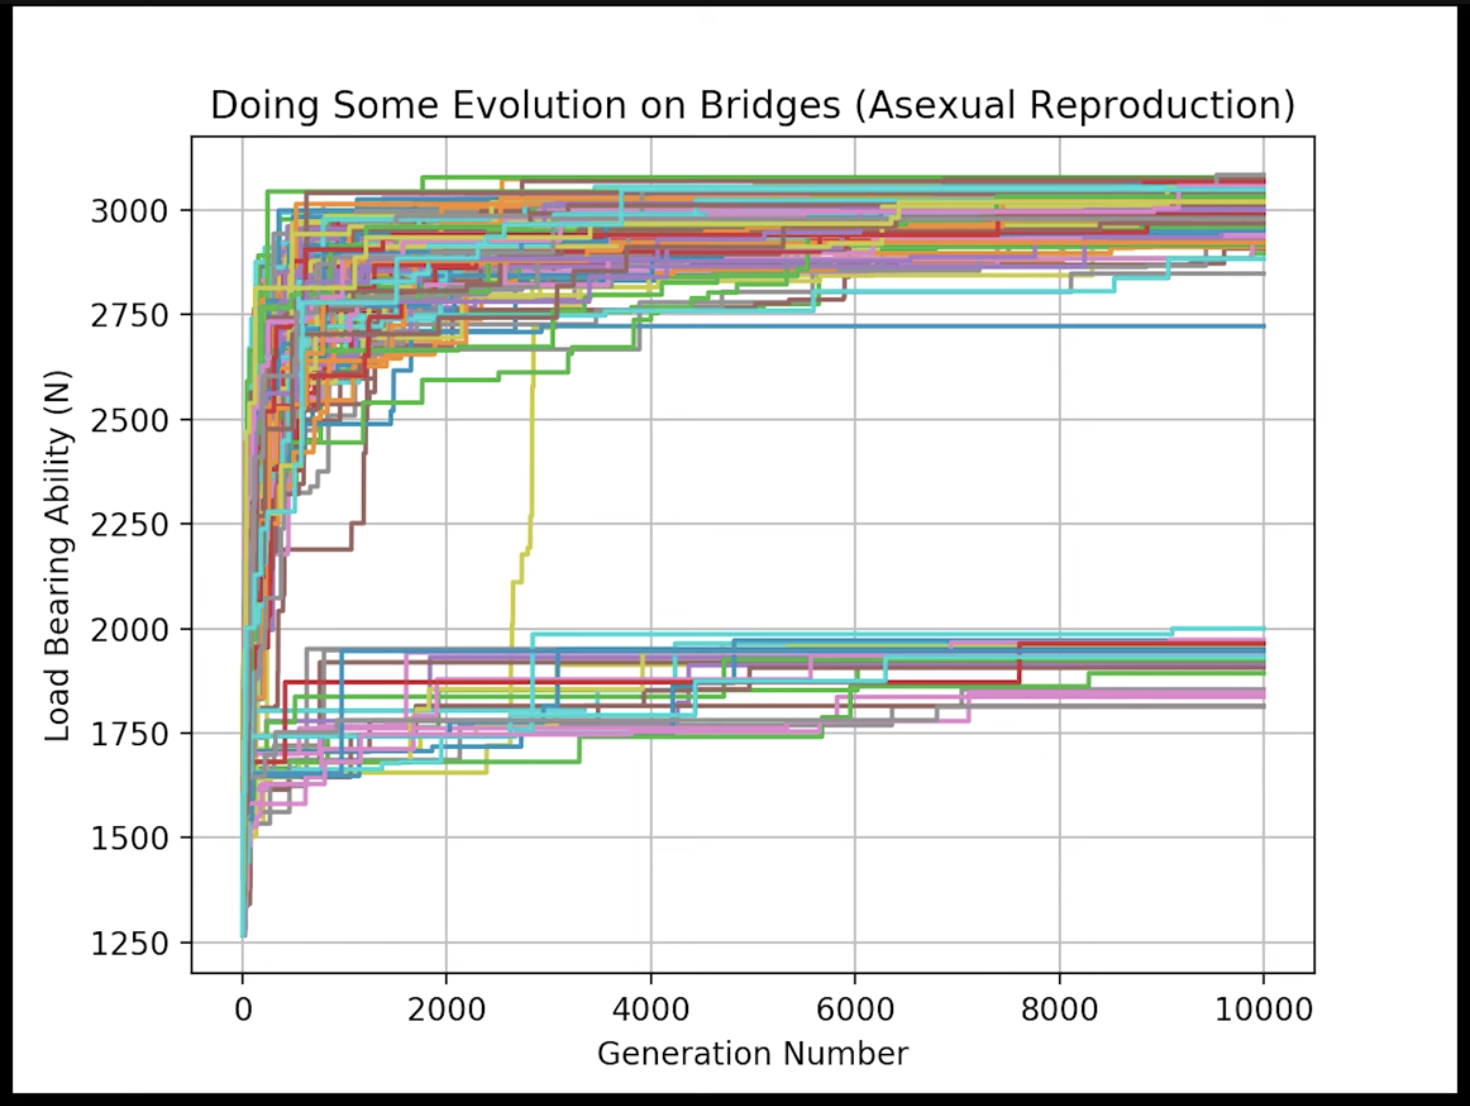
\includegraphics[width=0.7\textwidth]{img/image006.png}
\caption{As I documented this project, I learned the importance of goood data visualization and documentation for a project. In this case, it allowed me to learn that the solution space to the CIV102 bridges gave rise to two \textit{species} that can be seen on this graph.}
\label{}
\end{figure}

\subsubsection{Holistic Review}
From this project, I learned the importance of having a firm grasp on the {mathematics, science, history} behind any given opportunity. If I didn’t know the formulae for bridge failure loads, there would have been no way for me to create the genetic algorithm. Furthermore, in the words of Professor Collins, “one must know the answer before they solve the problem” - we would not have been able to make a good expected value calculation if we didn’t know how other teams had fared in the past (i.e. the history).

\subsection{Praxis II Launcher}
This project was refreshingly short-term compared to the last two. The underlying principle was also significantly simpler - the formulae we initially applied were readily apparent from our PHY180 course, and there was no underlying sociological/psychological literature to catch up on.

\begin{figure}[H]
\centering
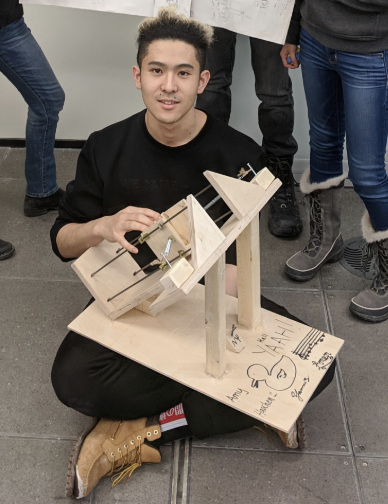
\includegraphics[width=0.7\textwidth]{img/image007.png}
\caption{The final launcher - note the solid building techniques, construction, and design for accuracy.}
\label{}
\end{figure}

\subsubsection{Process}
Since this was such a short-term project, we didn’t follow any given design model in particular. Instead, we started with a \textbf{solo to group brainstorming} session, and from then argued for each of our overall ideas. Every argument we made was tied to our main objective of getting the highest mark possible (i.e. getting the highest accuracy possible). That was our ground from which we made our claims. We used this productive \textbf{team argumentation} flow to narrow down our conceptual design based on which one we thought had the best chance of getting the ball accurately into the box, and then we argued over the engineering sub-decisions such as which fasteners to use and what type of projectile to use (in a similar manner to the \textbf{divide and conquer technique}). We began fabrication once we were satisfied that our design was optimized enough for the assignment.

\begin{figure}[H]
\centering
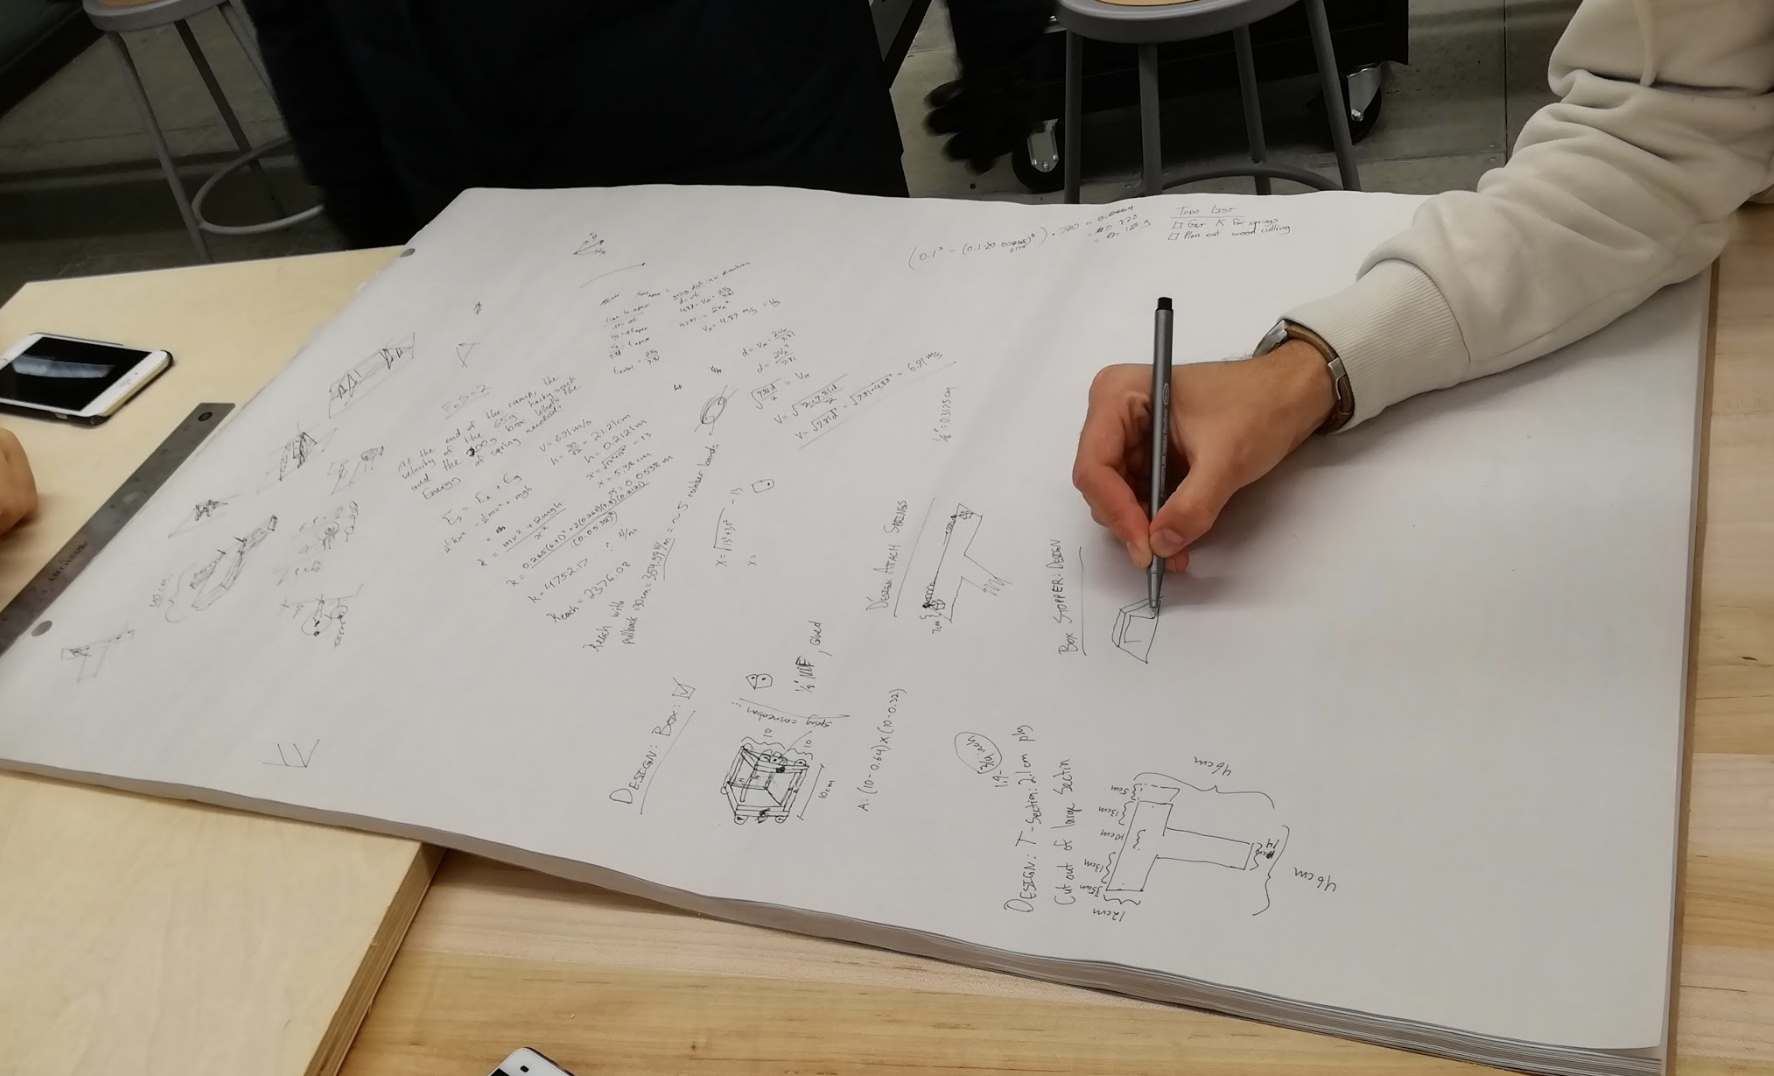
\includegraphics[width=0.7\textwidth]{img/image008.png}
\caption{Our recording sheet for our brainstoorming and team argumentation. It was a messy process, but the paper for rapid calculations and sharing of ideas was entirely necessary for our project to work as well as it did.}
\label{}
\end{figure}

\subsubsection{Holistic Review}
In the end, our design performed very well and only missed the target once in all of our trials. I believe that our argumentation process was a major contributor to this. We all had just finished PHY180 and CIV102 and therefore had a good grasp on the underlying concepts for building a launcher. This is what really enabled us to use the continuous \textbf{team argumentation} process to narrow down both our conceptual design and each of our small design decisions, as we all had a common ground upon which to stand when making our arguments. Our goal was clear along with our knowledge of how to reach it using PHY180 and CIV102 concepts and formulae.

\subsection{UofT Consulting Association Engagement: CareRelay}
I was a member of the UTCA SCG (University of Toronto Consulting Group Startup Consulting Group) from September 2018 to April of 2019. Our goal was to assist the company CareRelay with their healthcare apps’ onboarding, user retention, and user acquisition process. 

\begin{figure}[H]
\centering

\includegraphics[width=1\textwidth]{img/image009.png}
\caption{The companies description of our contribution to their product.}
\label{}
\end{figure}

\subsubsection{Process}
Helping this company involved a lot of research and a significant amount of reference design comparisons. As the only first-year student on the team and one of the few non-graduate students, I had to carefully consider my input to the team. I didn’t want to upset our group leader or make it seem like I knew better than them just because I am in engineering. However, I was able to implement some engineering design concepts that helped us in both coming up with our solutions and communicating them.
In almost all of our suggestions to the company, we \textbf{triangulated} our research with multiple companies, guides, and research papers. This enabled us to significantly increase our level of rigour and certainty in addition to our ethos with the company. Overall, triangulation was a highly valuable tool that improved our trust in our own suggestions as well as the companies trust us and our suggestions.

\begin{figure}[H]
\centering
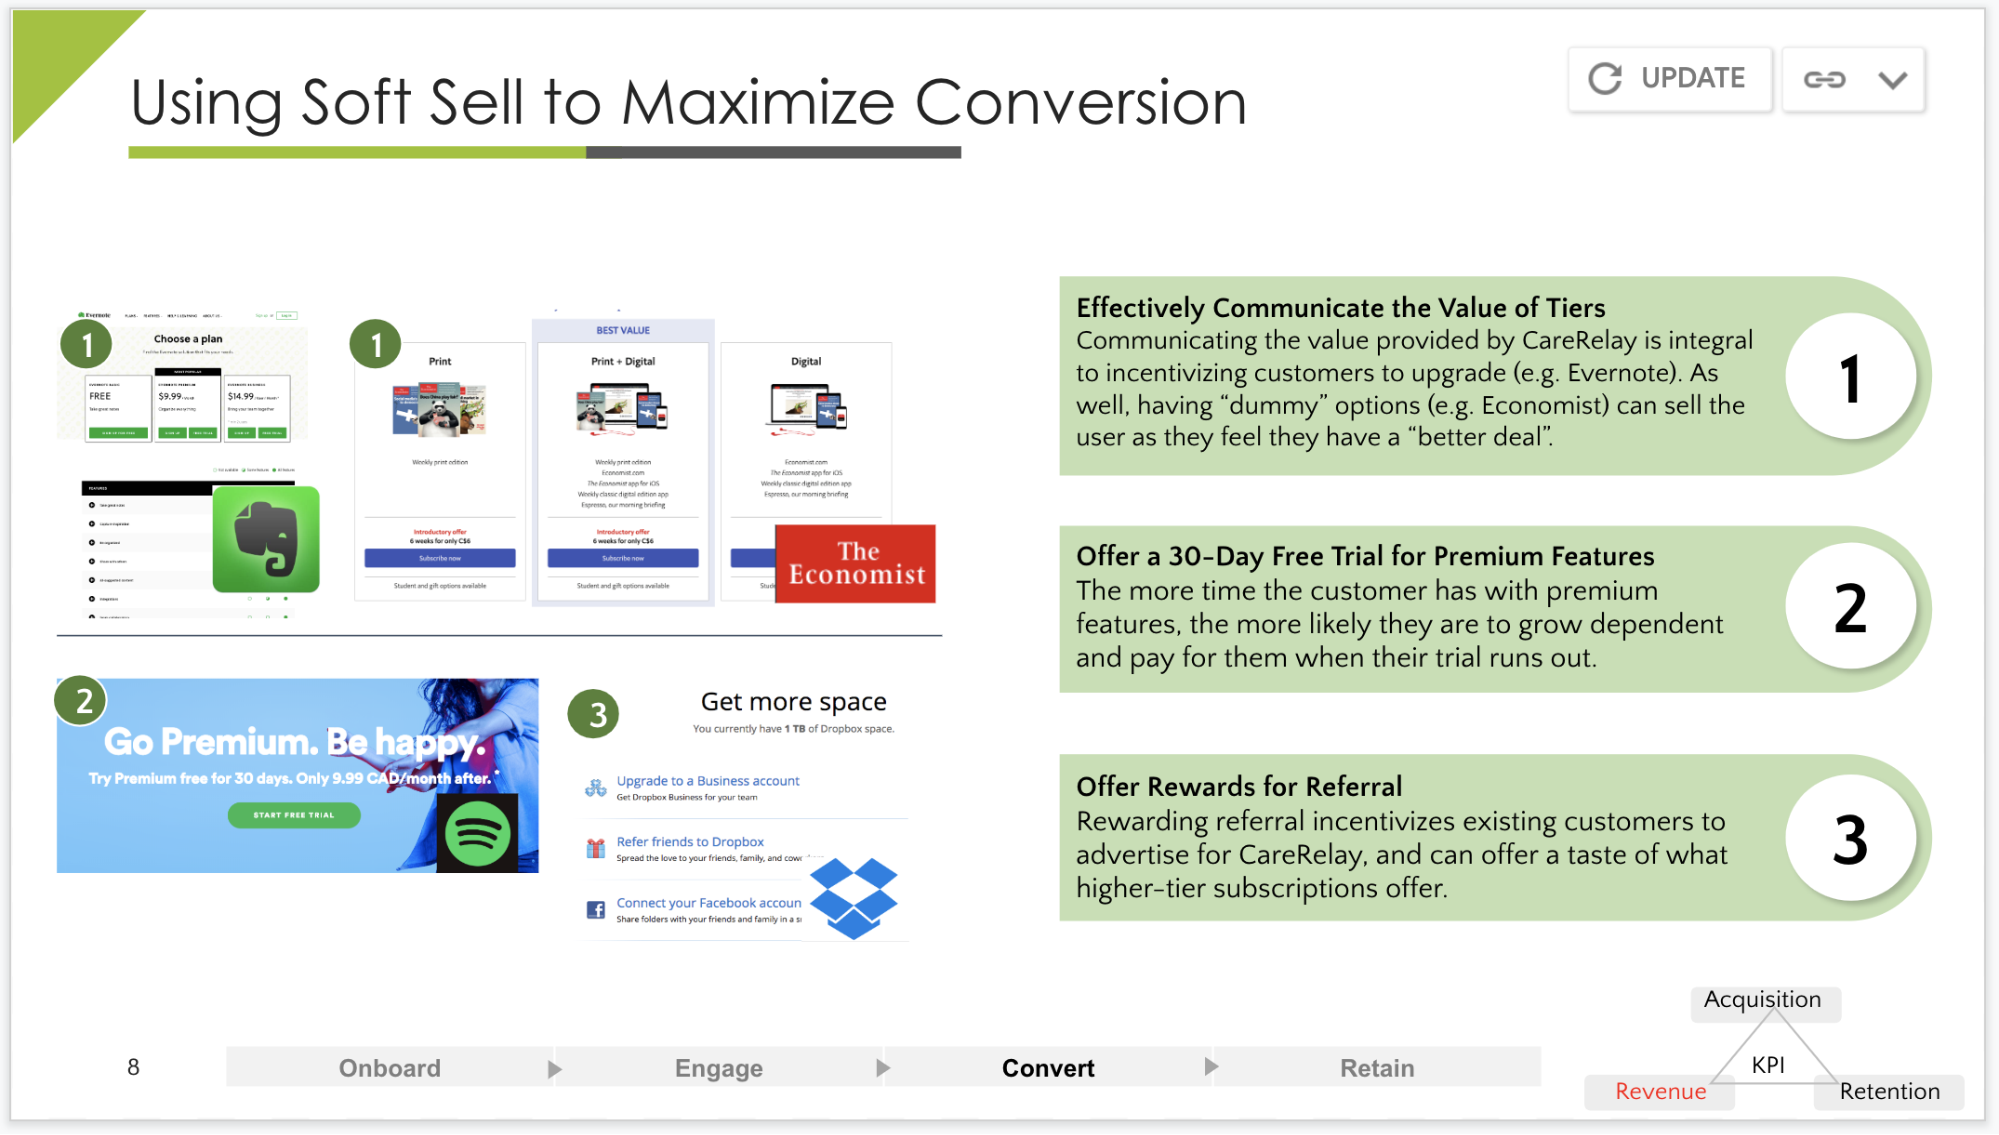
\includegraphics[width=1\textwidth]{img/image010.png}
\caption{Triangulation via referencing multiple companies' strategy to support a claim.}
\label{}
\end{figure}

One of the primary ways in which I did this was by encouraging the group to use a \textbf{how/wow/now matrix} to present our suggestions to the company. This essentially involves plotting each idea on the two axes of value and difficulty of implementation. The cluster that is high in value and low in difficulty of implementation are “wow” ideas, the ones high in value and high in difficulty of implementation are “how”, and the ideas low in value and low n difficulty of implementation are “now”. The client found this very useful, and they even referenced it in a job interview I recently had with them.

\begin{figure}[H]
\centering
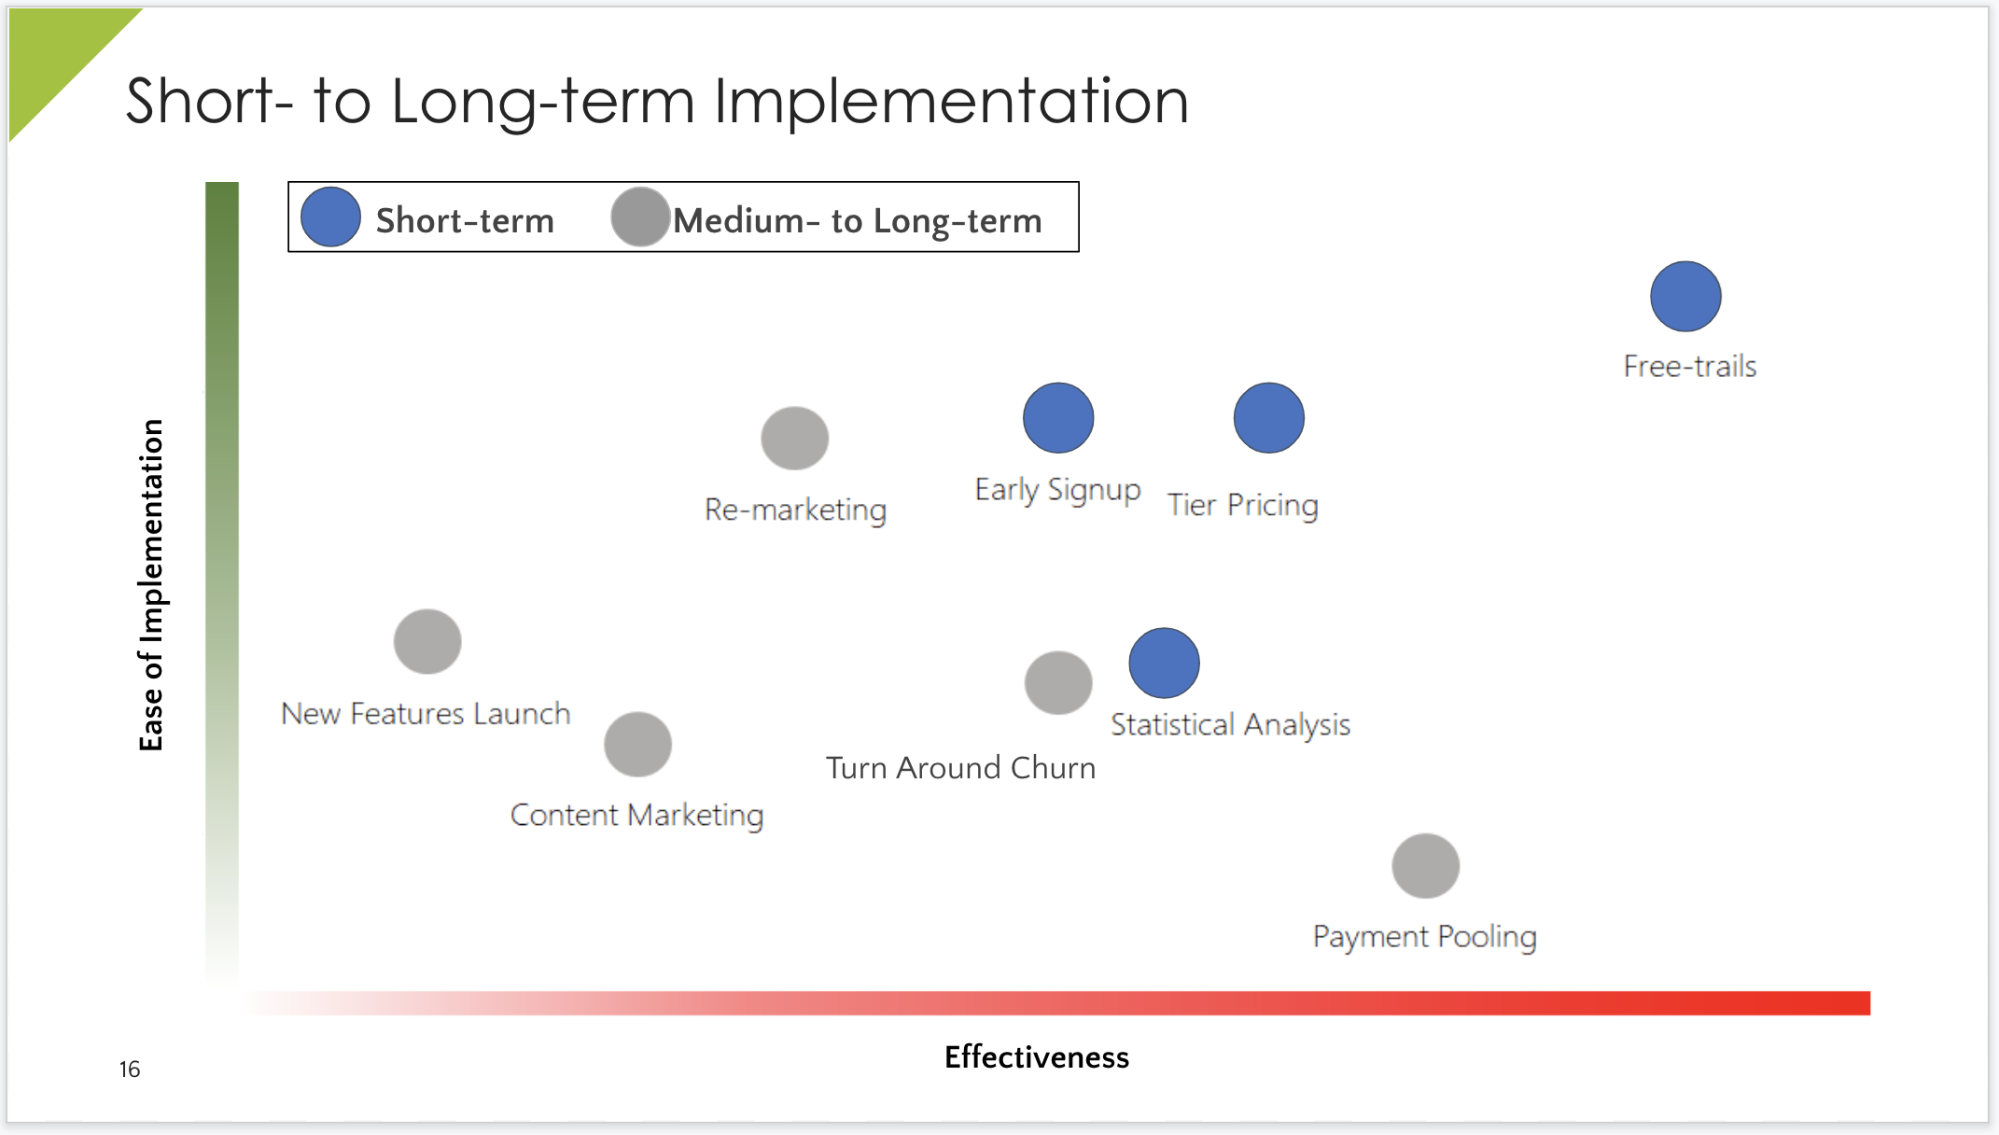
\includegraphics[width=1\textwidth]{img/image011.png}
\caption{How/wow/now matrix used in our final pitch to the startup. Closed our presentation well and allowed us to easily recap the ideas discussed and view their relative merits.}
\label{}
\end{figure}

\subsubsection{Holistic Review}
I believe that there is a lot of room in consulting to further implement engineering strategies to become more and more rigorous. The more tools in one’s toolbox one brings to an opportunity, the higher their chances of success. When it comes to ideas for understanding, generating, eliminating, and showing ideas, consulting is clearly an are that can always use more.

\subsection{Play the Orchestra (MakeUofT)}

I had the privilege of working with Eli Scott, Helen Newton, and Adam Carnaffan (all EngSci 2T2) at MakeUofT 2019, the largest makeathon in Canada, to actualize our idea of playing the orchestra. We created a product that allows a user to effectively play a live orchestra in real time via a MIDI keyboard. It takes in the MIDI data from the keyboard and intelligently routes each note of the chord to the screens in front of different members of the orchestra to be played. It also incorporates custom chord analysis and prediction software, in addition to a physical display unit that we build out of a Raspberry Pi. 

\subsubsection{Process}
We had just finished our first round of midterms, and it was the end of the week before reading week. We were all tired, but we forced ourselves to meet at a coffee shop the night before the hackathon. The theme of the hackathon was connectivity and internet of things, and since it was a makeathon, our minds were filled with ideas of swarm robotics and robots that could connect to sensors and more. Toward the end of our meeting, we tentatively settled on the idea of making a swarm of small robots that could intelligently assemble in order to move very large objects, assigning just enough robots to lift the object to increase efficiency over conventional forklift robots.

However, one of our team members, Helen Newton, was dubious of the feasibility of the project. She could not imagine building an entire swarm of robots that could communicate with each other and intelligently parse that data within 24 hours. Looking back on the process, it is clear that she was correct. At the time, however, it seemed like she was really playing \textbf{devil’s advocate}. She did this continuously for the duration of the meeting and continued to poke holes in the ideas as we tried to ammend our ideas to make them more feasible. This resulted in us picking the Play the Orchestra idea.

Once our idea was picked, we were ready to start developing the idea during the hackathon the next day. Since I was the only person on the team who had participated in a hackathon before and experience with the development side of things that would be required to develop our product, I was a primary planner for how we would tackle the problem. In my experience, teams who do well in hackathons tend to incorporate the sponsor’s technologies and have an interesting, flashy design that fits well with the theme of the event. I wanted our final solution to have those aspects, but I also wanted us to be able to have something to show for our work as quickly as possible. I remembered how, in a game development lecture from a UOIT student group, they discussed the concept of a \textbf{MVP (Minimum Viable Product)}. A good MVP communicated the key functionality of the product with the least possible work. My plan for creating our final product was to get that done as soon as possible then add to it as time went on.

\begin{figure}[H]
\centering
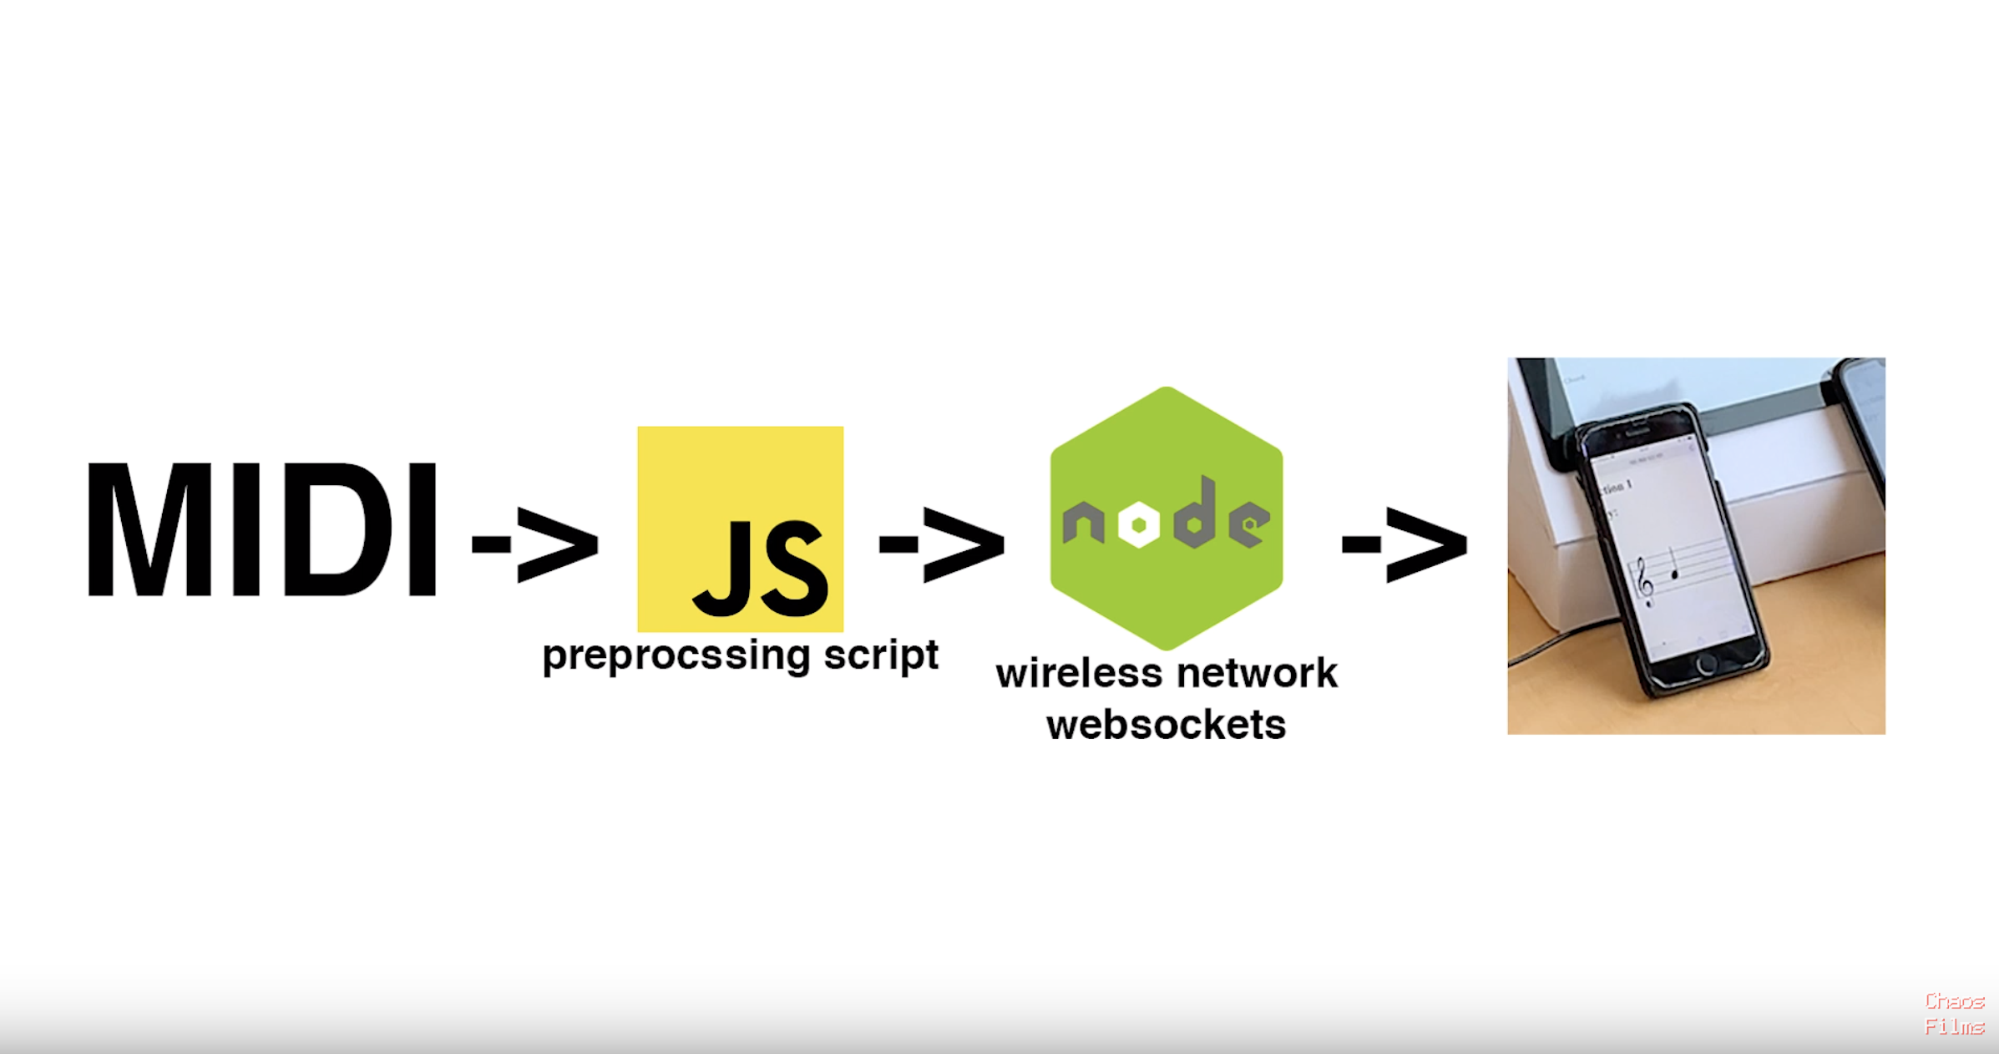
\includegraphics[width=1\textwidth]{img/image012.png}
\caption{Path of information in our Play the Orchestra system. This constituted our minimum viable product (MVP), a tool discussed at length later on. This design was fairly simple but enabled us to grow the prduct to a winning design.}
\label{}
\end{figure}

Within 4 hours, we had a system that could read 4-note MIDI chords from a keyboard and send it through a custom, low latency network to 4 separate devices. With our remaining ~18 hours, we worked to improve the following:

\begin{itemize}
	\item Aesthetics (showing a proper note staff)
	\item Chord analysis
	\item Intelligent chord prediction/suggestion (using sponsored tech, Azure ML)
	\item Making a physical device with a Raspberry Pi (to fit better with the internet of things as opposed to just having a software version)
	\item Scalability of our general operation (from quartet to an orchestra)
	\item Polish our documentation (using sponsored tech, hackster.io)
	\item Testing our product with real musicians
	\item Creating our submission video
\end{itemize}
In the end, we won third place overall (competing against teams of 4th year students) as well as prizes for best documentation. We came out with several thousand dollars with of tech from sponsors.

\begin{figure}[H]
\centering
\includegraphics[width=0.4\textwidth]{img/image013.png}
\caption{Myself, Helen, Eli, and Adam with some of our prizes.}
\label{}
\end{figure}

\subsubsection{Holistic Review}

Helen playing the \textbf{devil’s advocate}, as well as our use of the \textbf{MVP} framework really drove our success in the hackathon. I also think that the importance of a solid team dynamic where each person trusts that the goal of each other person is to advance the project is import, along with a hierarchy of believability that each person can use to decide the degree to which they ought argue/accept each claim made by others in each domain of the project. For example, I readily gave into claims made by Adam when it came to networking because he had the most experience and expertise in the field and was therefore the most believable by far. Only if I were very sure of my reasoning and facts would I argue against his claims. Likewise, Eli was the most believable when it came to finding the best way for us to document and describe our process due to her clear competence in the field based on her past achievements and success in Praxis I. This sort of \textbf{believability-weighted decision making} is very important and valuable for making good decisions quickly and taking advantage of each person’s expertise on a given team.

I would also like to point out that, in the lecture in which he introduced the idea of an MVP in engineering design, Prof. Foster referenced our documentation for our hackathon project [1].

\subsection{Praxis II Firefighter RFP Implementation}
For our Praxis II project, Amy, Haochen, Yannis and I worked on the firefighters RFP that requested a solution to the lack of situational awareness in firefighting.

\subsubsection{Process}
We picked our RFP based on how interesting we thought it would be to work with the stated group and how interesting it would be to work on their problem. The most interesting one to us by far was working with firefighters on situational awareness. Firefighters have important and interesting jobs and situational awareness has a lot of potential to be improved by engineering and technology.

We began by scoping outward from the RFP because we felt that the requirement for our solution to help with both pathfinding and situational awareness really pushed toward a very specific type of situational awareness. After scoping out to just situational awareness, we did some research during the studio where we were supposed to be using “as many tools as possible” in order to diverge, much to chagrin of Professor Patricia Sheridan. We did this because we felt that we didn’t have enough of an understanding of the field from the RFP in order to properly diverge well. We thought our \textbf{pareto curve} would be optimized if we were to research and then diverge. Once we felt we had enough research to do some effective diverging, we did some \textbf{multi-panel diverging} on the provided whiteboards. This was highly effective as it allowed us to \textbf{creatively recombine} various ideas, and we were able to literally take a step back from the board when we wanted to think in a more big-picture way and recombine ideas and take a step toward the board when we wanted to expand on one particular idea. We came up with three main ways to help the firefighters with situational awareness:

\begin{enumerate}
	\item Incorporating gas sensors into each firefighter’s suit to localize the fire/classify the type of fire.
	\item Incorporating physiological sensors into the firefighter’s suits to track the cardiovascular health of each firefighter over time. 
	\item Creating an optimized version of the entry control board to minimize human error.
\end{enumerate}

\begin{figure}[H]
\centering
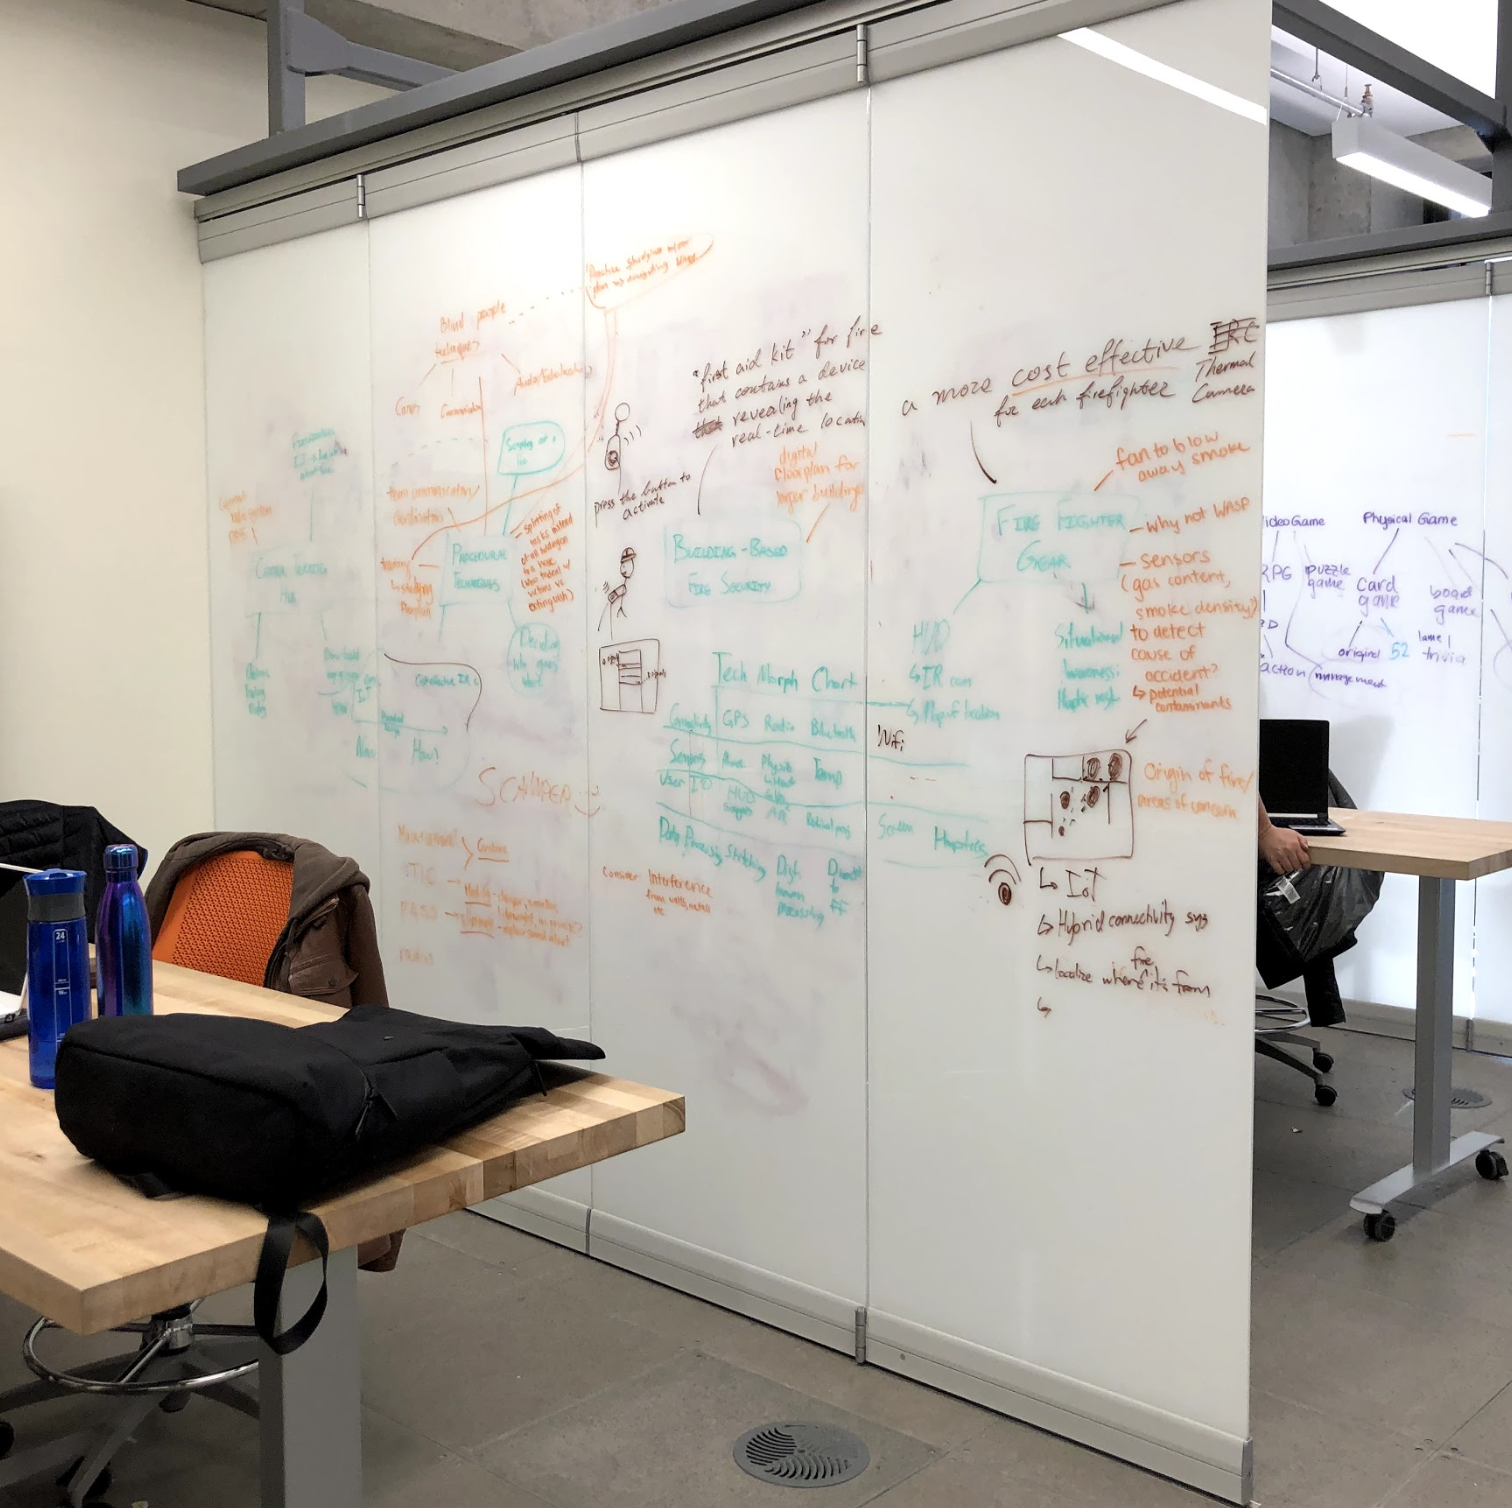
\includegraphics[width=0.65\textwidth]{img/image014.png}
\caption{Our 4-panel breadth-first diverging setup. Note the activity at the intersections of the panels (this was soome of the most valuable in the process)}
\label{}
\end{figure}

\begin{figure}[H]
\centering
\includegraphics[width=0.65\textwidth]{img/image015.png}
\caption{Two of our resulting prototypes (gas and physiological sensors). These prototypes enabled us to be very sure of our choice to narrow down to entry control as our opportunity later on, and they existed thanks to our multi-panel diverging process}
\label{}
\end{figure}


When we had our first stakeholder interaction, they were fairly neutral when it came to the first two ideas, but they really liked the last idea about entry control. We created prototypes for each of them to get a better sense of what it would be like to actually implement them, and we presented our work at beta. We used \textbf{multi-vote} to narrow down to just the entry control board idea, and then used \textbf{sensitivity analysis} to confirm our choice. The multi-vote was very effective because the team’s interest and belief in the idea was an important quality for our project, and the sensitivity analysis enabled us to confirm that our mental models for evaluating the situation were consistent with a numerically encoded and agreed upon model of that same situation.

\begin{figure}[H]
\centering
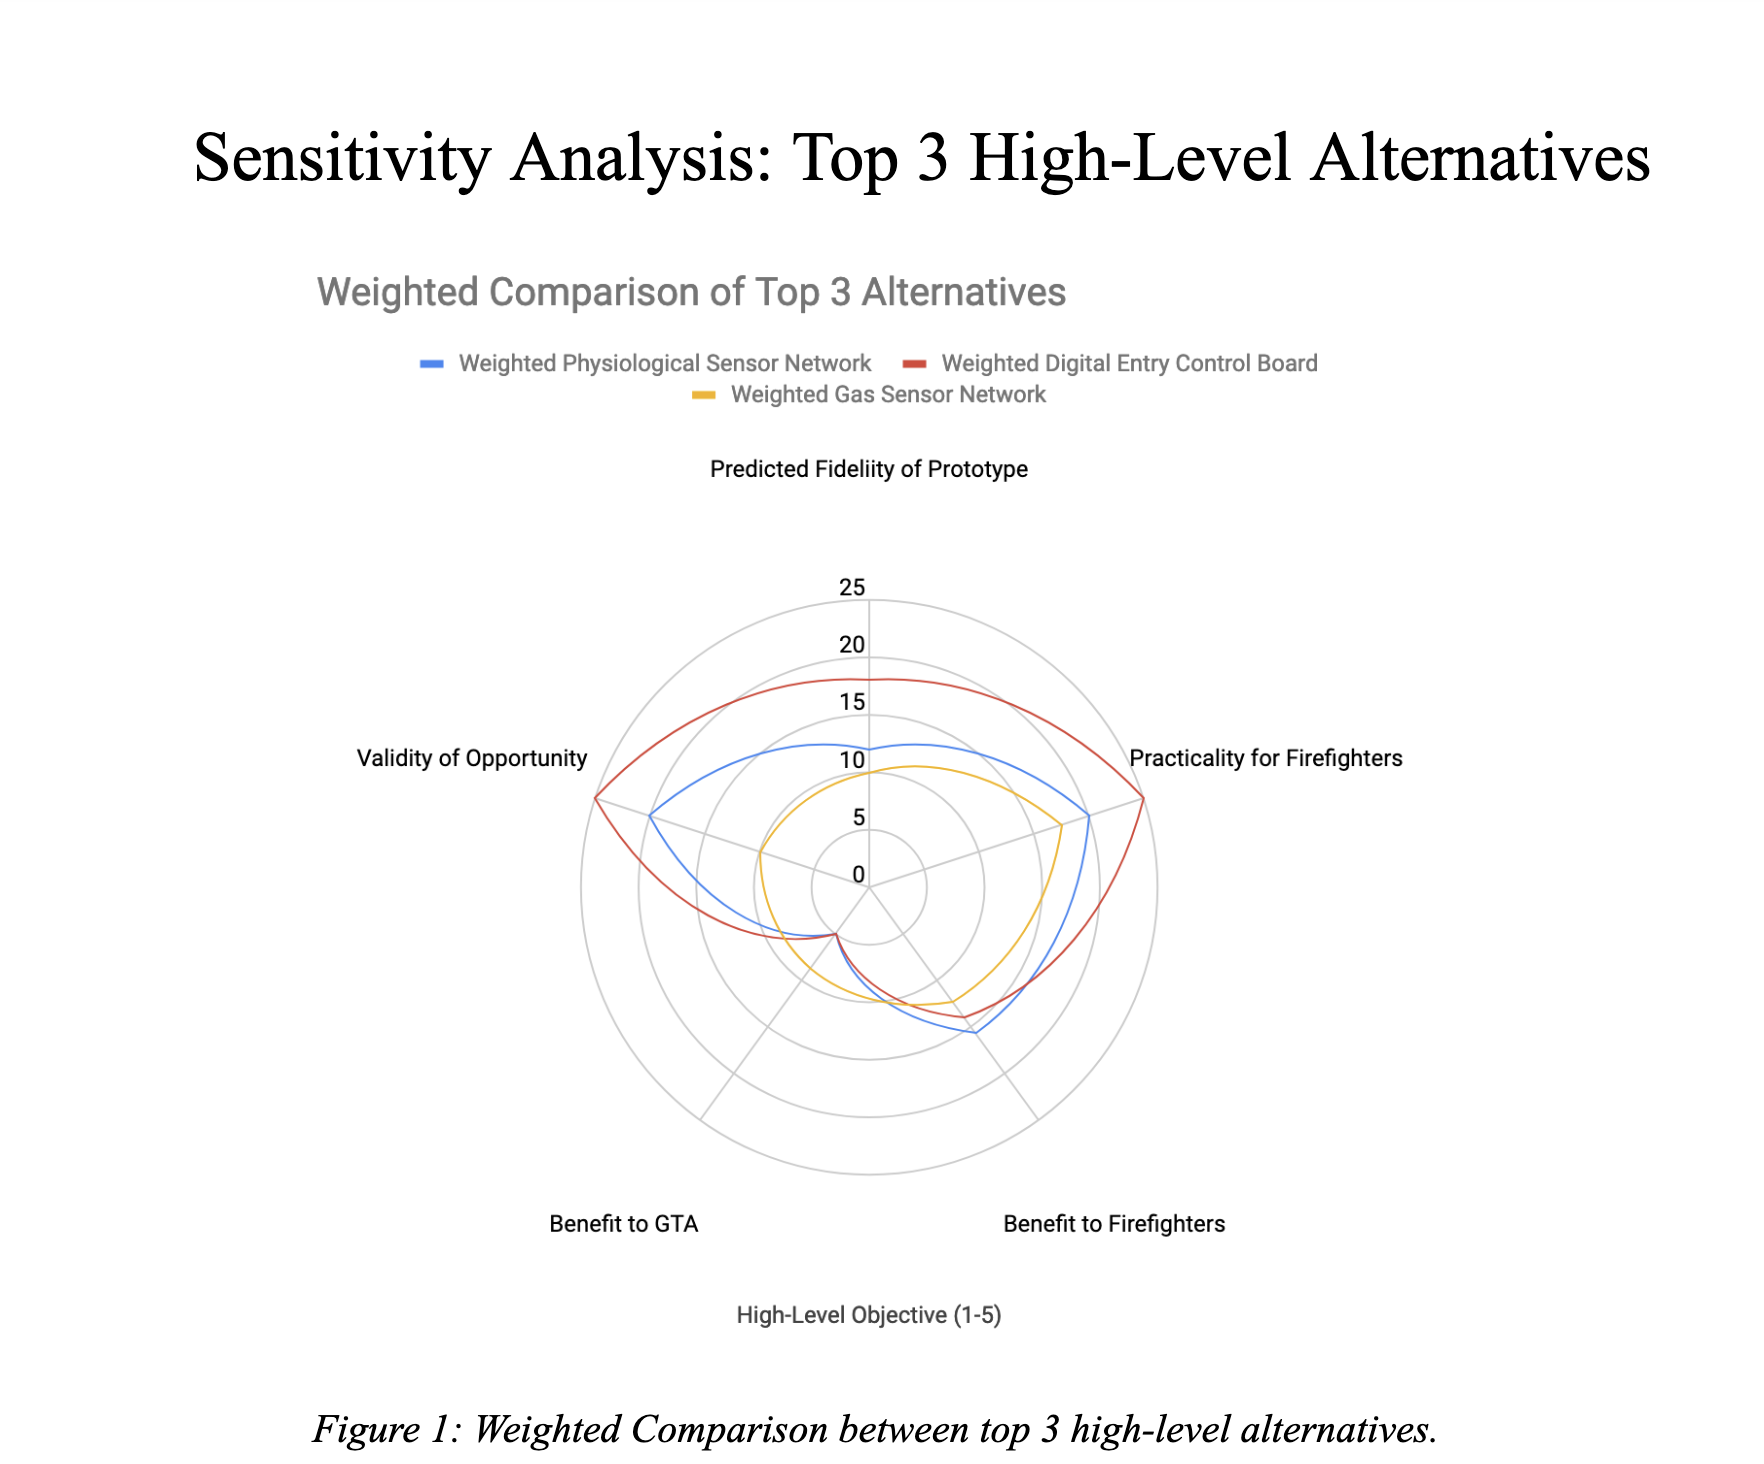
\includegraphics[width=0.9\textwidth]{img/image016.png}
\caption{Our sensitivity analysis was highly effective in communicating why we made our decision to converge as well as in confirming our initial multi-vote and intuitive feelings on the matter.}
\label{}
\end{figure}

We had very positive feedback from our beta release, and it was at this point that we started on our more intense UI, cognitive load, and human error research to create our UI requirements model. Taking an idea from the famous Steve Jobs, a titan of design, we created our first rough prototype using the \textbf{shoshin} approach; we did no research beforehand and simply tried to generate what an entry control board ought to look like from first principles. It is a technique that essentially minimizes anchoring bias. Our shoshin prototype formed a great basis for our \textbf{iterative design} process. Our second prototype took a small step towards realism by incorporating some of our research.

\begin{figure}[H]
\centering
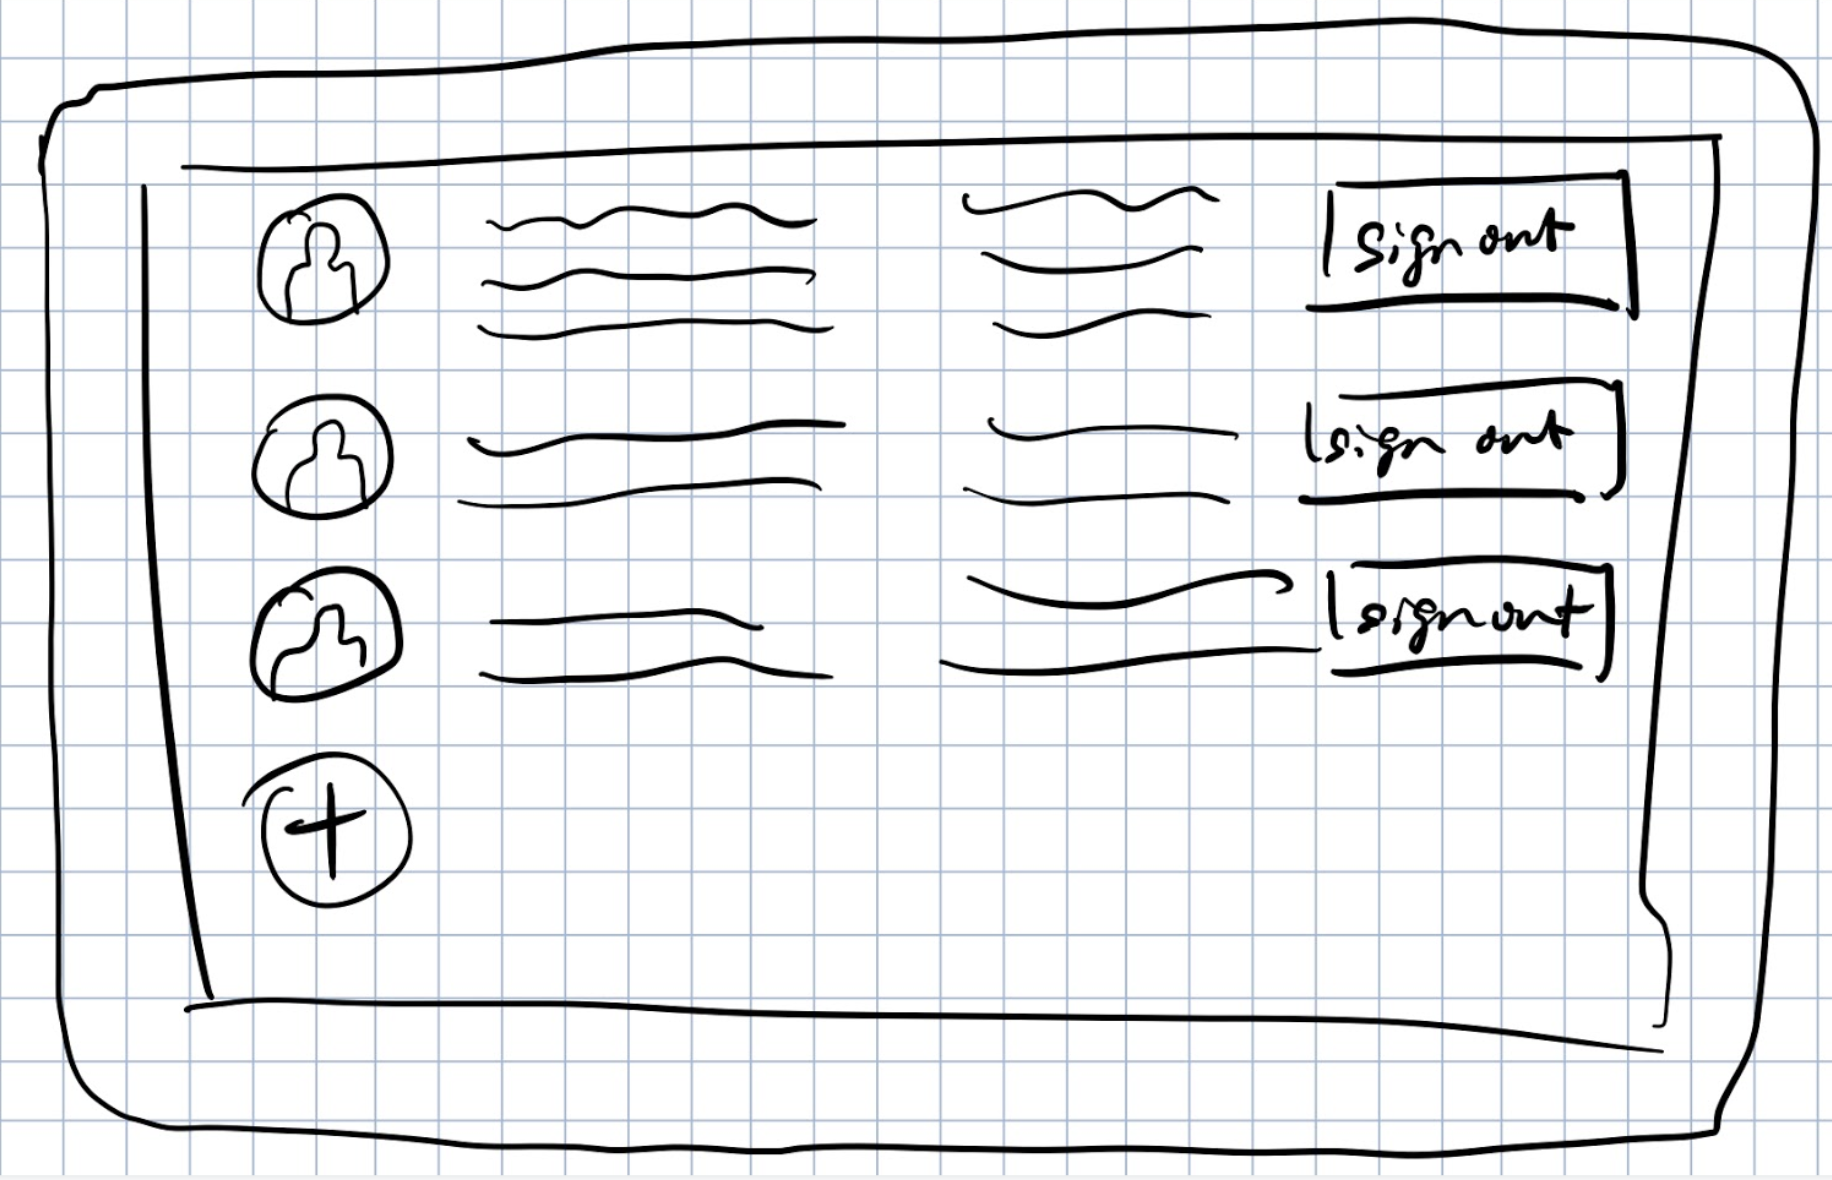
\includegraphics[width=0.4\textwidth]{img/image017.png}
\caption{The shoshin prototype was very quick and low-quality, but it we felt that it reduced our anchoring bias overall because our starting point for iteration was not affected by the status quo.}
\label{}
\end{figure}

At this point I began work on our third version that would hopefully be testable. It was a barebones version of an entry control board where every team and option was already hard-coded in. It functioned as an \textbf{MVP} for our testing and showcase, as well as a proof of concept that the javascript library Angular.js could accomplish all the things we wanted from our digital entry control board.

\begin{figure}[H]
\centering
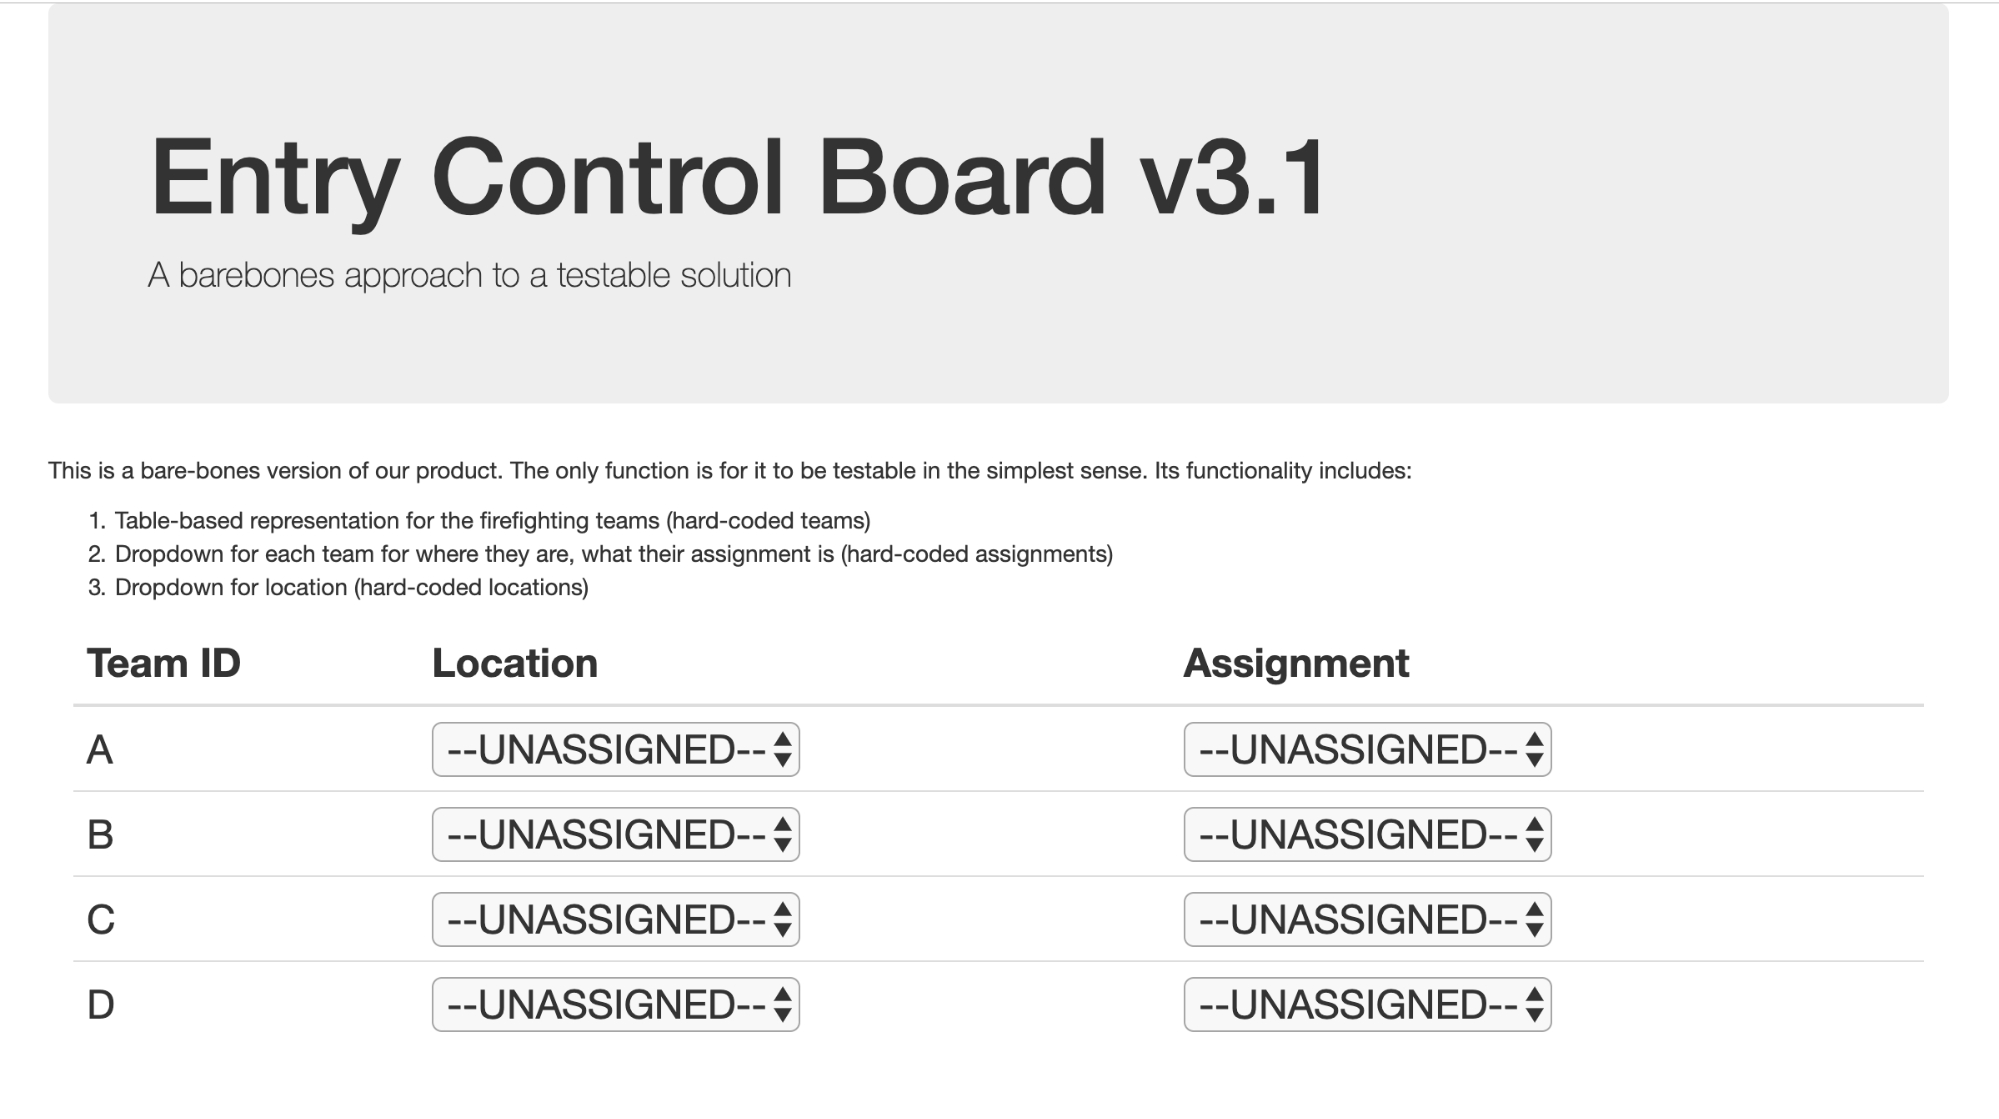
\includegraphics[width=0.7\textwidth]{img/image018.png}
\caption{A more testable prototype that still retains many elements from the shoshin version.}
\label{}
\end{figure}

From version 3.2-3.5, I iterated our design with the help of our UI requirements model, team feedback, and test user feedback. This process is what enabled us to move from a barebones, testable prototype to a fully functional prototype that had fantastic results with both validation with respect to our key metric of accuracy and with our stakeholder validation from real firefighters in station No. 315. The process also made it very easy to see what our next steps ought to be based on our requirements model and feedback from our stakeholders on our relatively highly actualized version.

\begin{figure}[H]
\centering
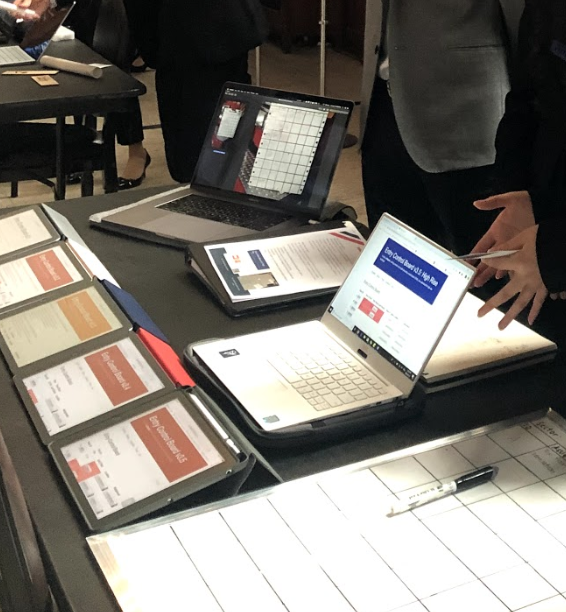
\includegraphics[width=0.7\textwidth]{img/image019.png}
\caption{Our line of iPads each running versions 3.1-3.5H on them was very effective in communicating the rigour of our process to the audience at showcase. Special thanks to Prof. Foster for offering the iPads.}
\label{}
\end{figure}

Meanwhile, we made a separate set of requirements for an improved analogue board to address more immediate issues from our stakeholder interactions. In order to make engineering sub-decisions, we used pugh charts to decide on such elements as which clock to use, which board type, which pen type, and more.







\end{document}
